\documentclass[twocolumn]{article}[h]
\usepackage[utf8]{inputenc}
\usepackage{graphicx}  % Required for including images
\usepackage{lipsum}    % This package generates fake text
\usepackage{geometry}  % For adjusting margins
\usepackage{titlesec}  % For customizing sections
\usepackage{url}  % Add this line to use the \url command
\usepackage{booktabs}
% Set the margins
\geometry{
  left=17mm,
  right=17mm,
  top=15mm,
  bottom=15mm
}

% Set the format for the section titles

\title{Band Structure for Fourteen Semiconductors}
\author{Hoang Nguyen\\
  Universite de Bourgogne\\
}

\begin{document}

\maketitle

\section*{1. Introduction}

This report examines the pseudoformfactors and band structures of 14 semiconductors: AISb, CdTe, GaAs, GaP, GaSb, Ge, InAs, InP, InSb, Si, Sn, ZnS, ZnSe, and ZnTe[1].

The approach involves the computational reproduction of band structures for these semiconductors, specifically focusing on face-centered cubic (fcc) structures. The study employs empirical pseudopotentials, a method renowned for its accuracy and efficiency in crystalline solid state physics. The Brillouin zone paths are meticulously mapped to ensure a thorough exploration of the electronic states.

The aim is to compute, analyze these band structures and compare my findings with the landmark study by Cohen and Bergstresser. This comparison is critical in validating the computational methods used.

\section*{2. Methods and Numerical Calculations}

The computational methodology commences with the definition of unit vectors in reciprocal space, which facilitates the construction of the reciprocal lattice vector \( \mathbf{G} \). The qpath for each band, sourced from the \texttt{BZpath} file, aids in assembling the reciprocal lattice. Subsequently, the potential \( V \) for each semiconductor is determined. This involves expanding \( V \) in terms of the reciprocal lattice vectors \( \mathbf{G} \), and incorporating the pseudopotential form factors \( V_G \):

\begin{equation}
    V_G = V^{S}_{|G|^2} \cos(\mathbf{G} \cdot \mathbf{s}) + iV^{A}_{|G|^2} \sin(\mathbf{G} \cdot \mathbf{s})
\end{equation}

For the calculation of form factors, Table 1 from Cohen and Bergstresser's study is utilized. However, given the dataset's origination in 1966, some of its data may not be fully refined, potentially leading to slight misalignments in the band structures.

Notably, in Cohen and Bergstresser's original dataset, \( V_0 \) was omitted. As such, after ascertaining the energy levels for each material, the maximum value of the third band is taken to the Rydberg scale, in accordance with the data presented in Table 1.

The pseudopotential Hamiltonian for the crystal includes both kinetic and potential components:

\begin{equation}
    H = -\frac{\hbar^2}{2m}\nabla^2 + V(\mathbf{r})
\end{equation}

Following the evaluation of all \( V_G \) values, these are incorporated into the Hamiltonian matrix. The kinetic energy is also computed and added into the Hamiltonian. The band structures for 16 materials are then derived by diagonalizing this Hamiltonian, encompassing both kinetic terms and pseudopotentials.

\section*{3. Results and Analysis}
\vspace{-1cm}
\begin{figure}[htb]
    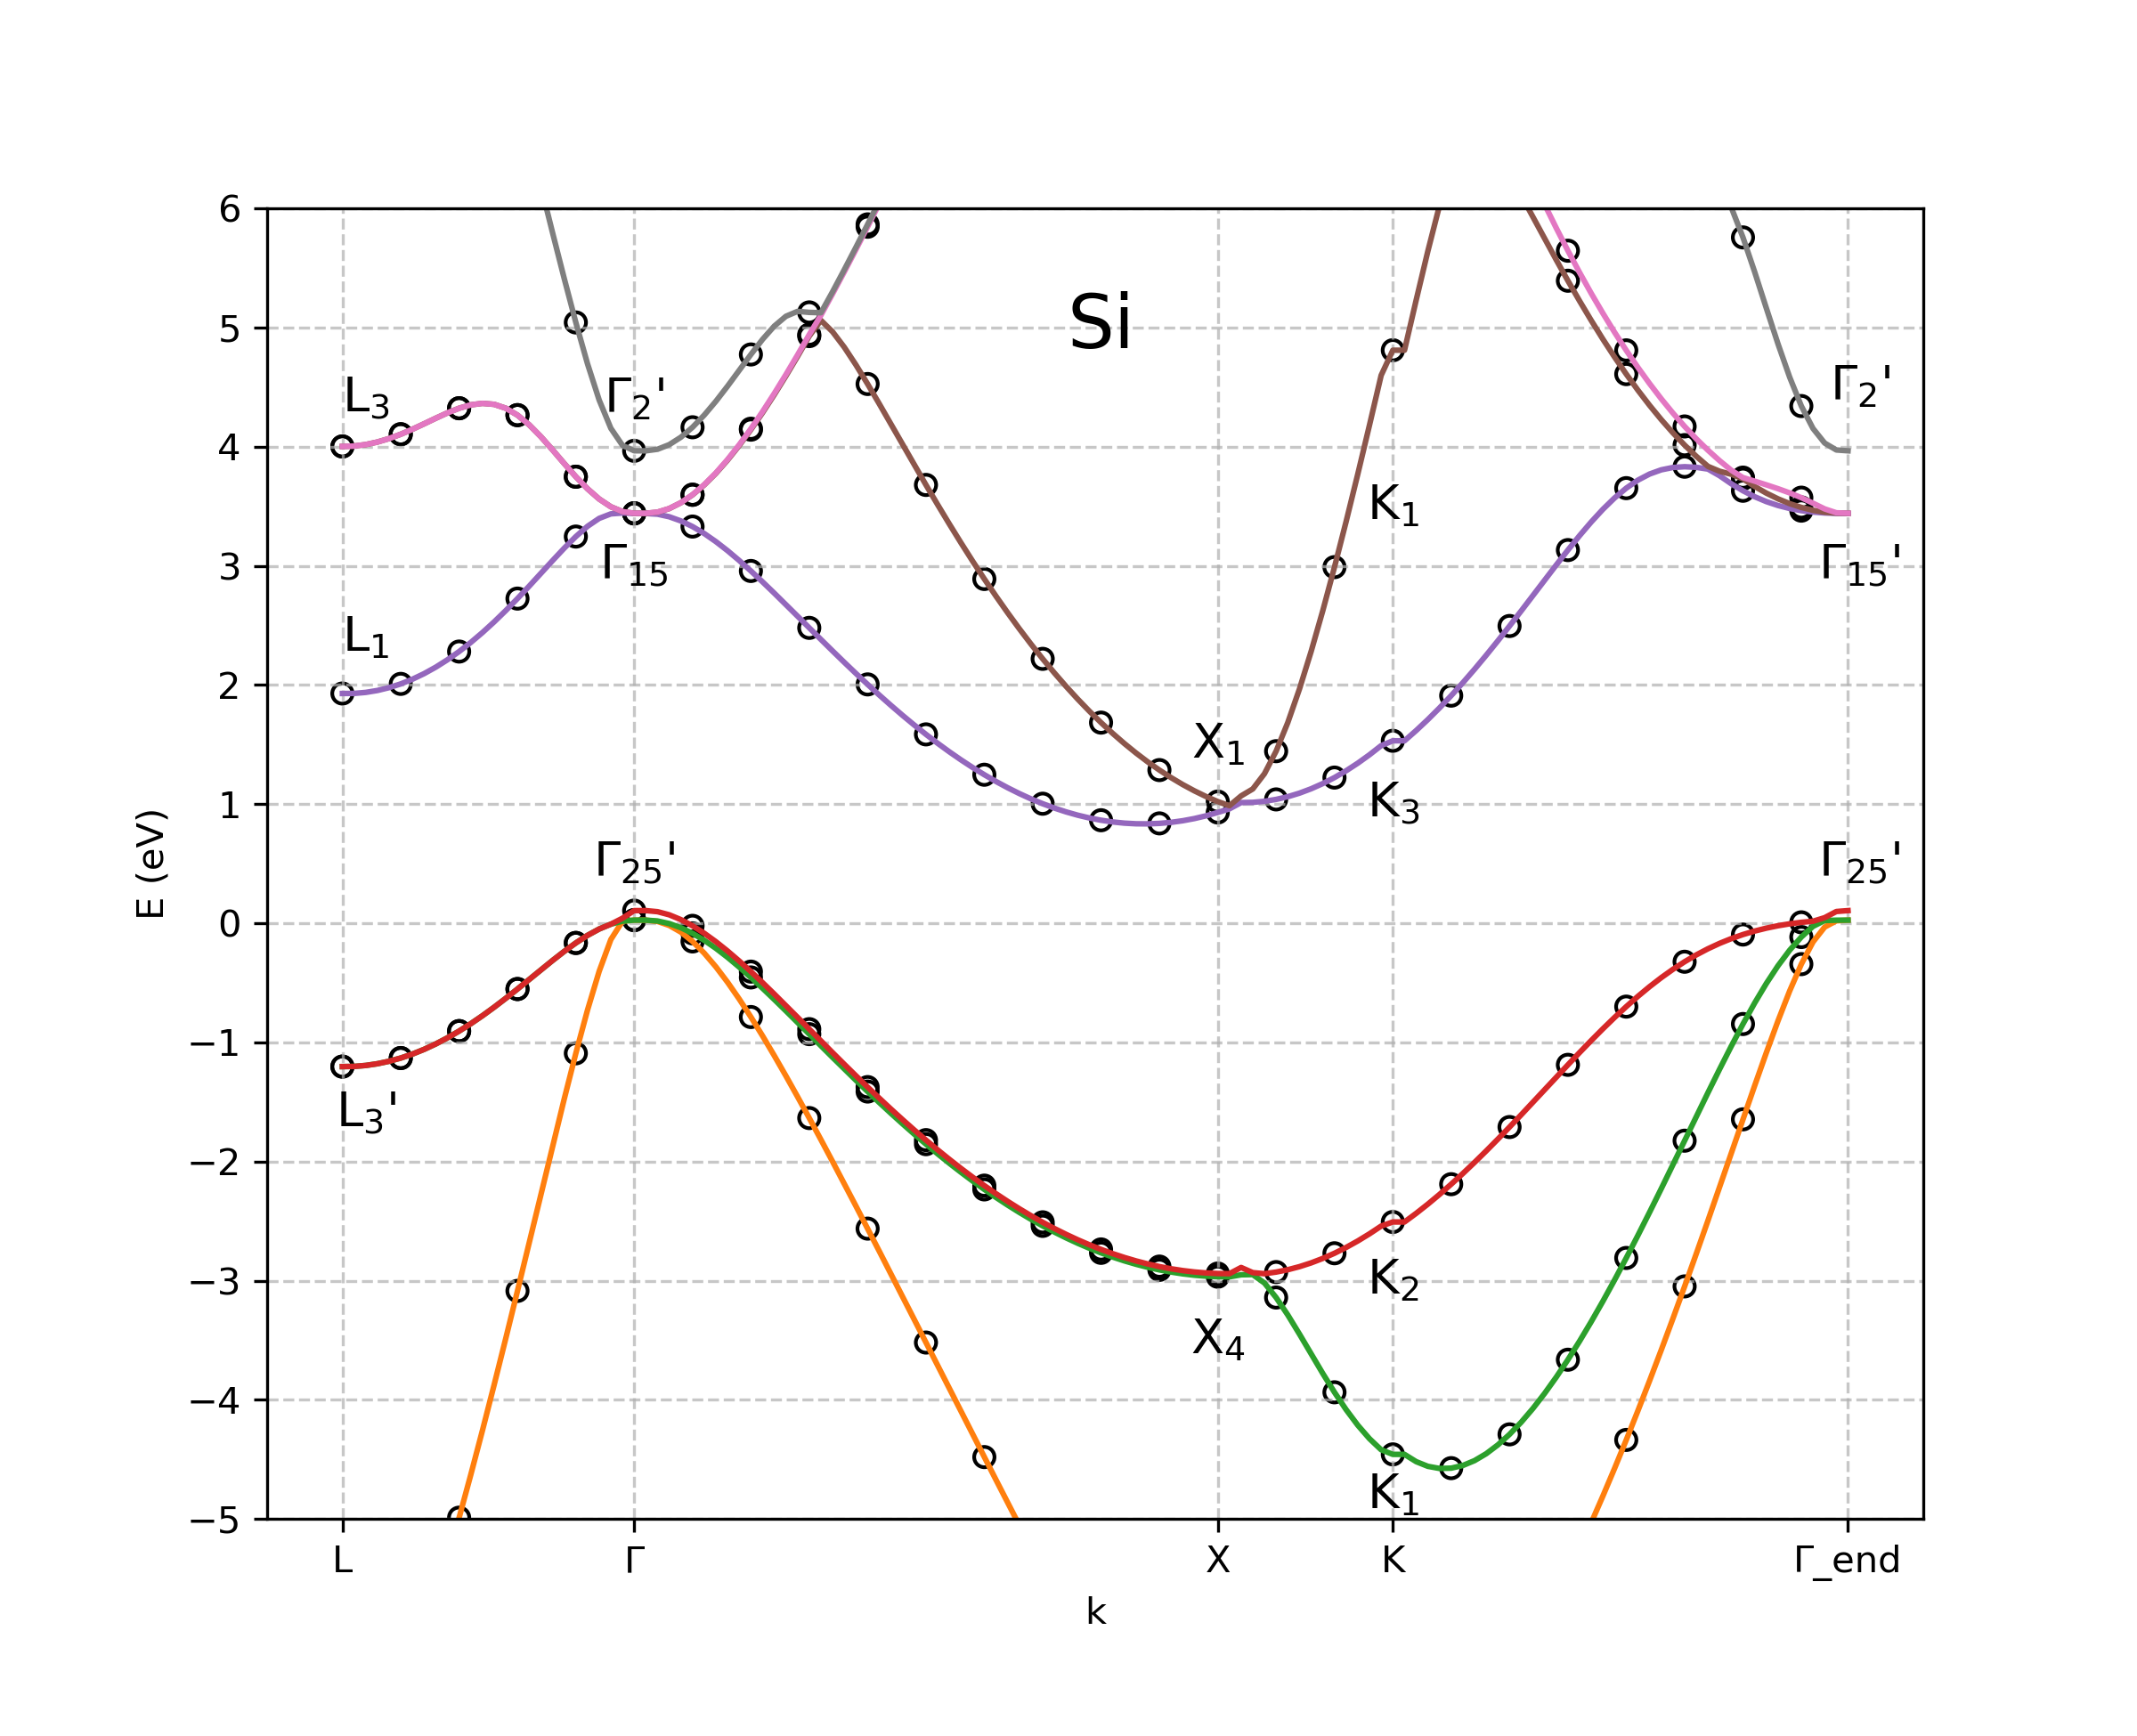
\includegraphics[width=\linewidth]{Si.png}
    \vspace{-1cm}
    \caption{Band structure of Si.}
    \label{fig:Si}

    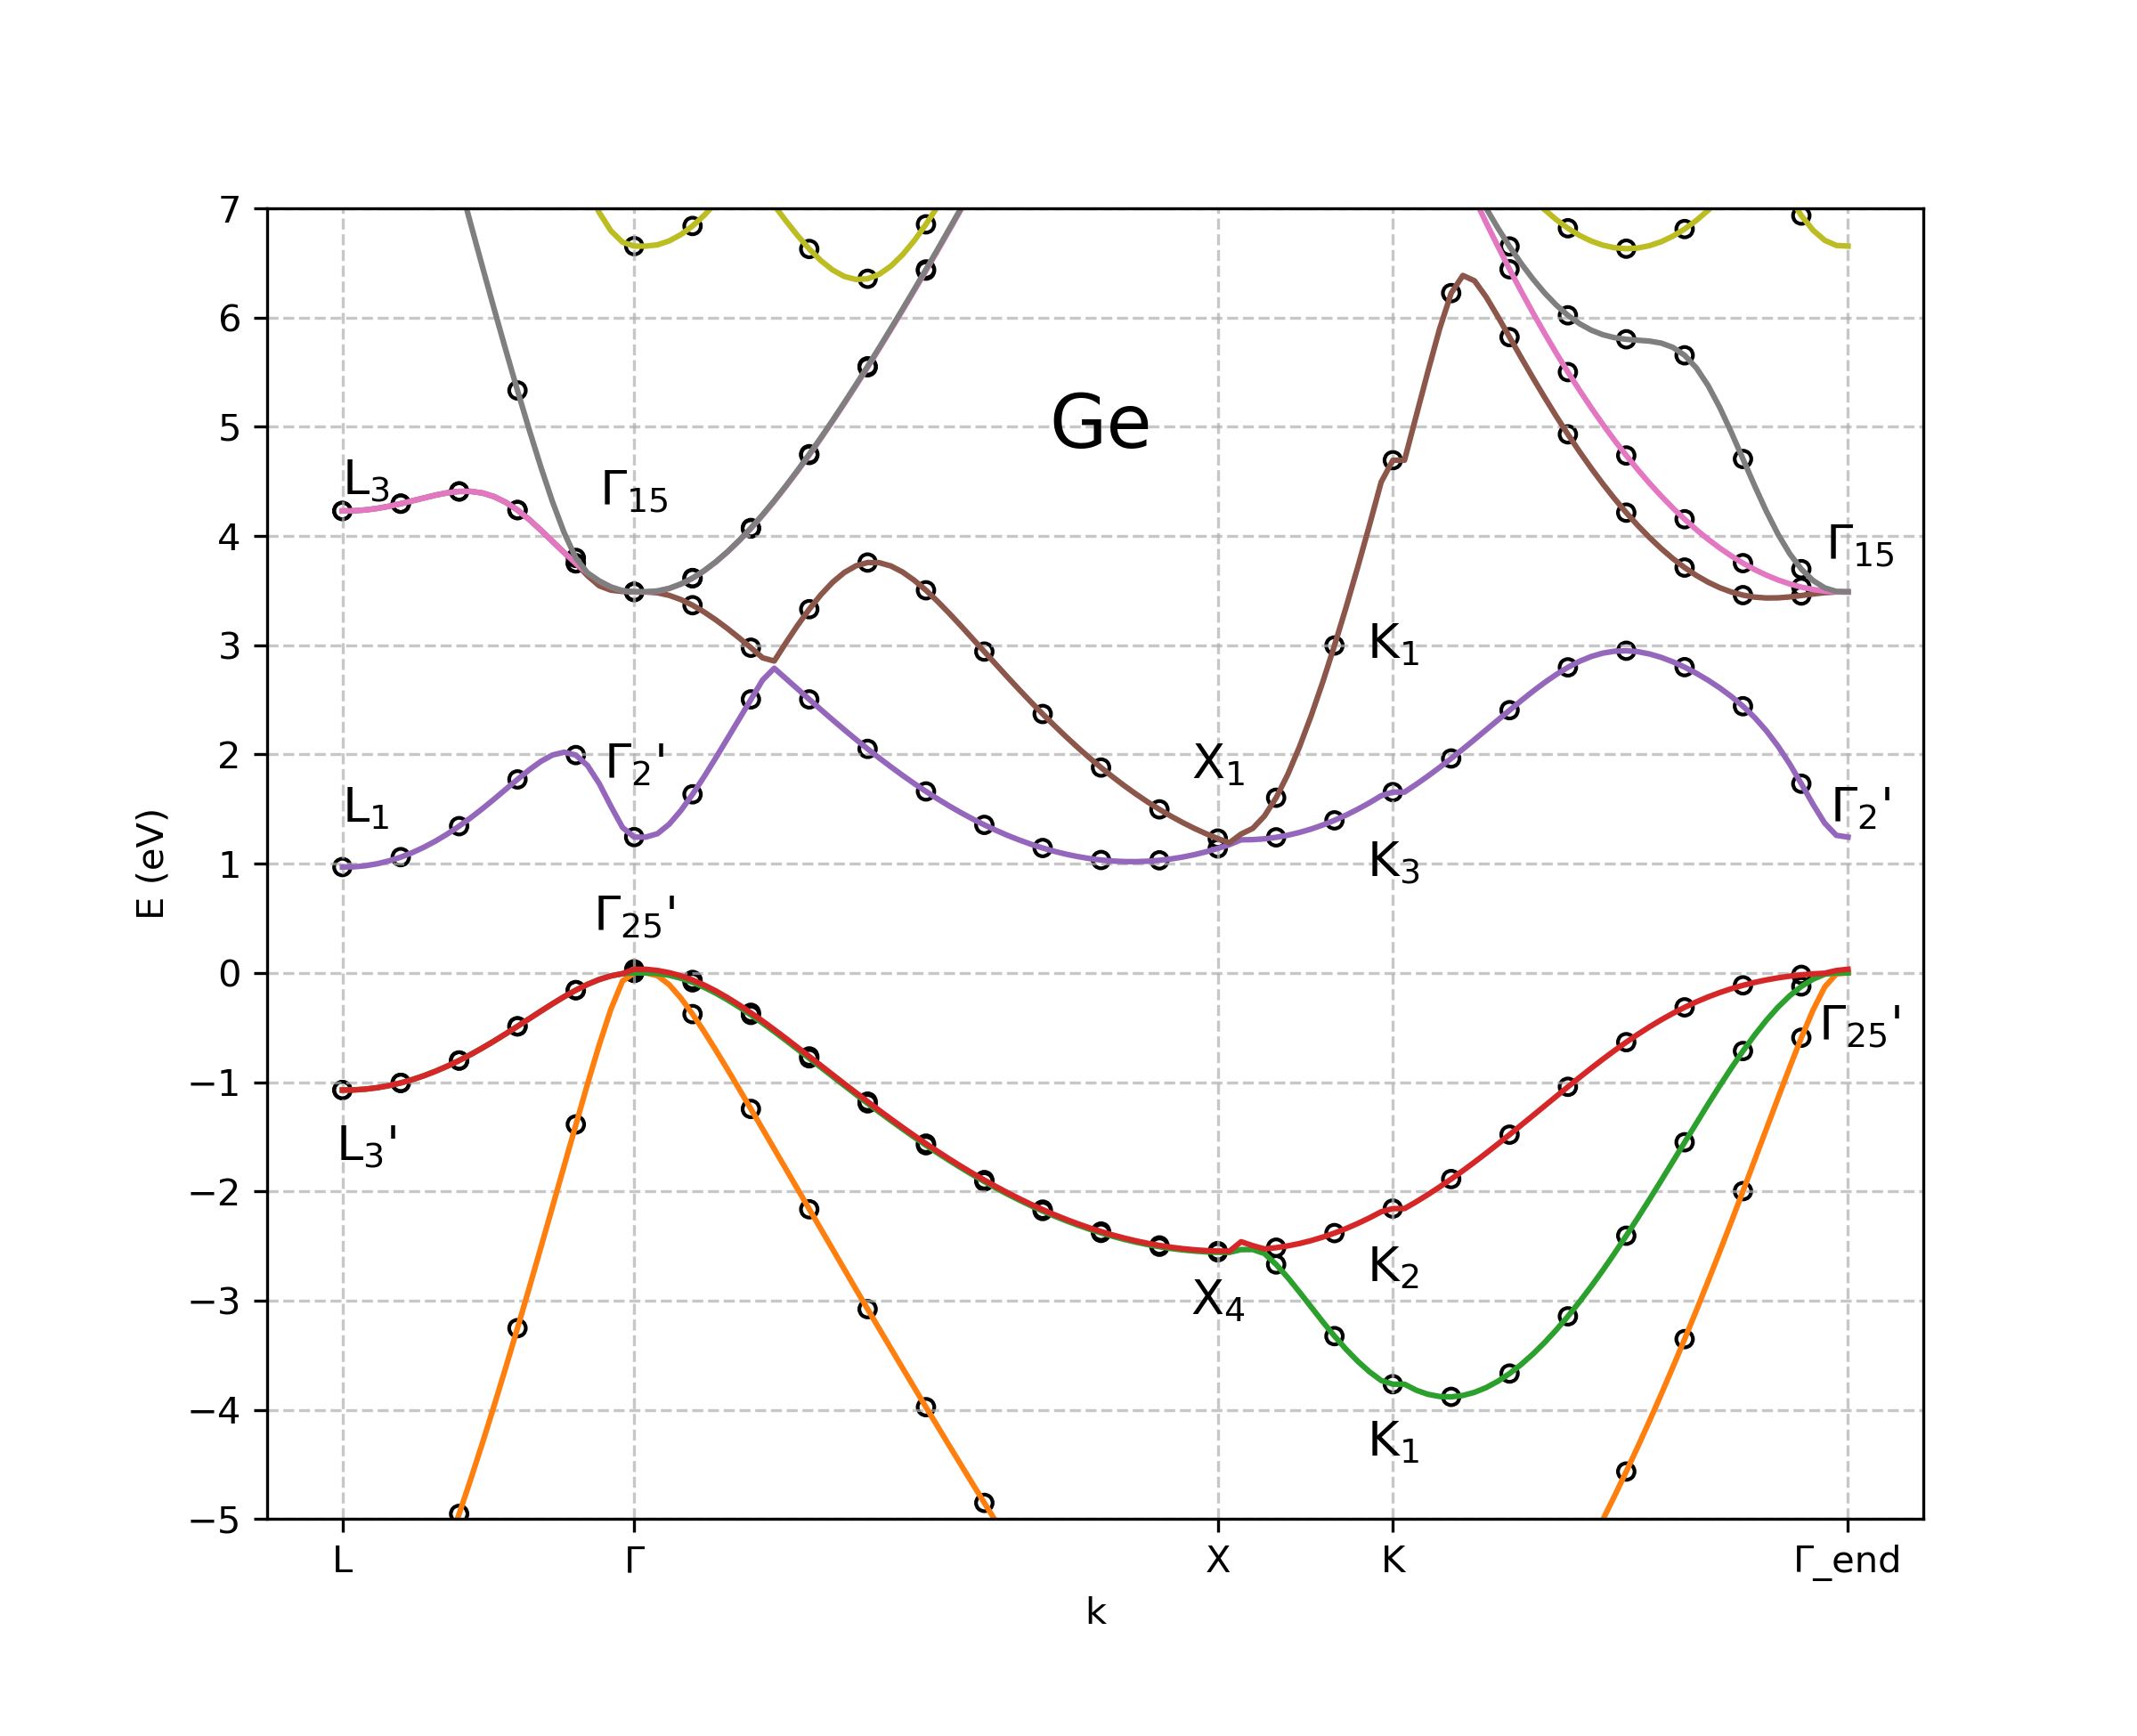
\includegraphics[width=\linewidth]{Ge.png}
    \vspace{-1cm}
    \caption{Band structure of Ge.}
    \label{fig:Ge}
\end{figure}

\begin{figure}[htb]
    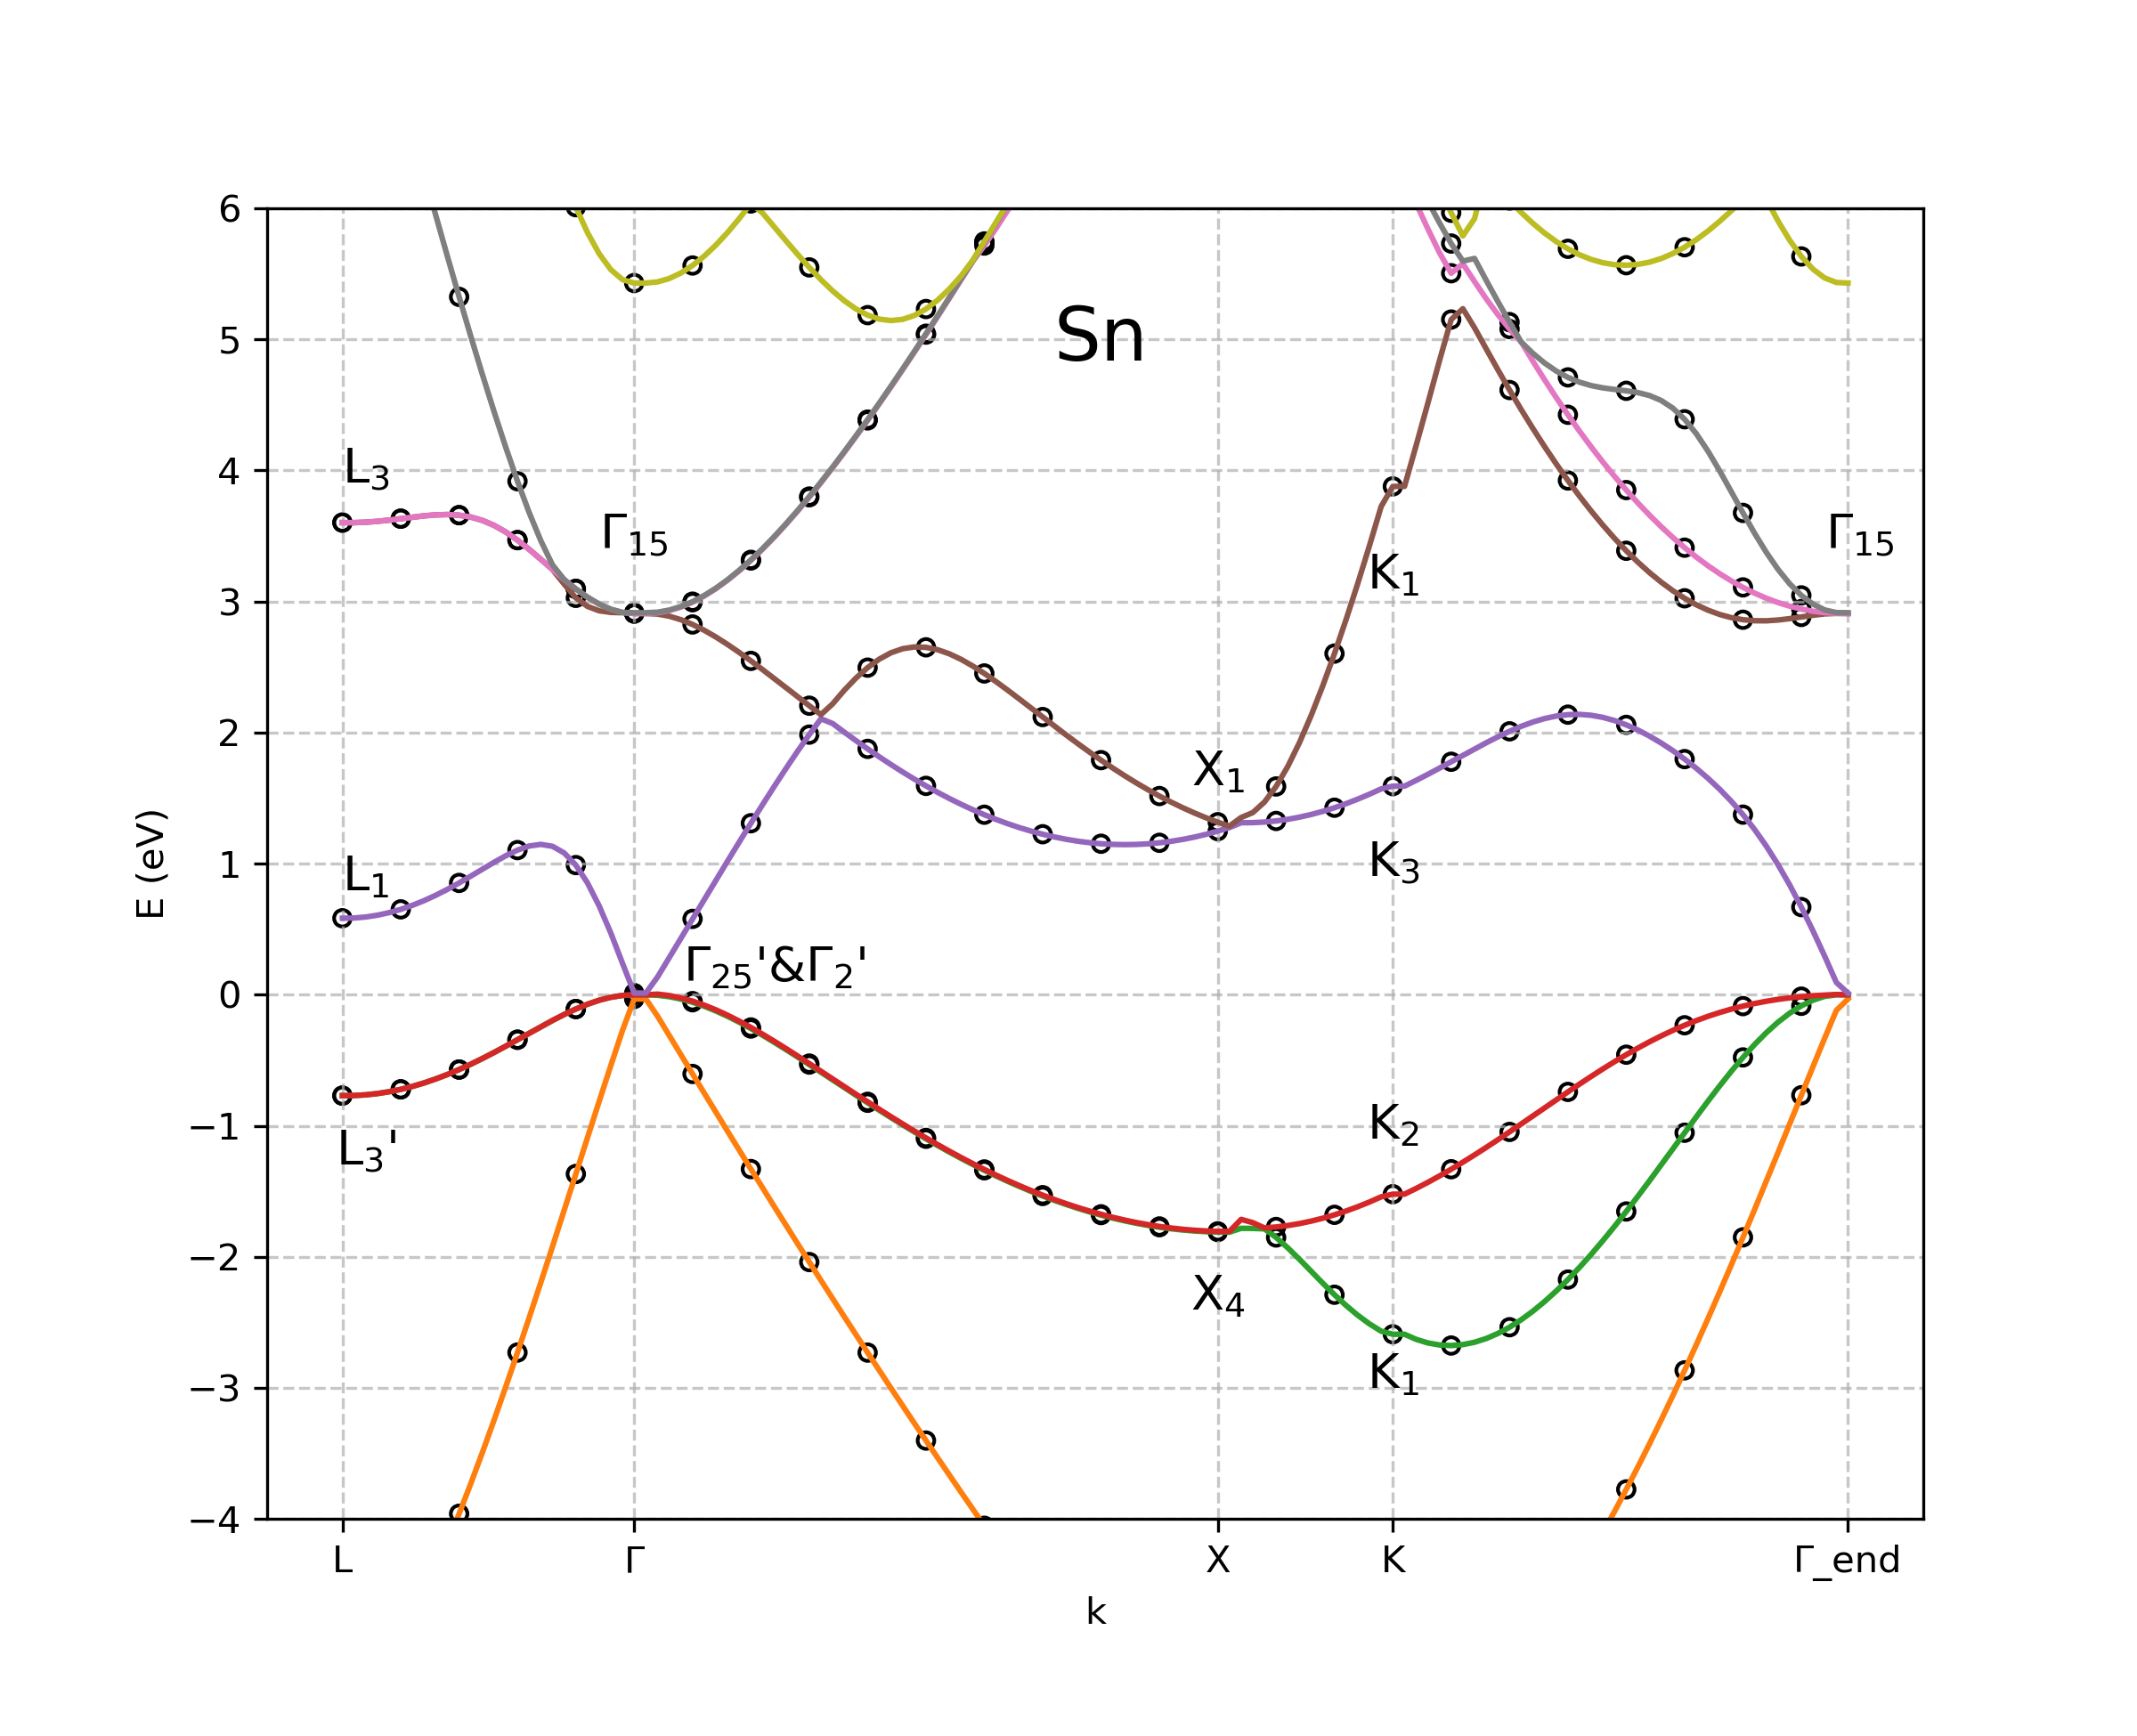
\includegraphics[width=\linewidth]{Sn.png}
    \vspace{-1cm}
    \caption{Band structure of Sn.}
    \label{fig:Sn}

    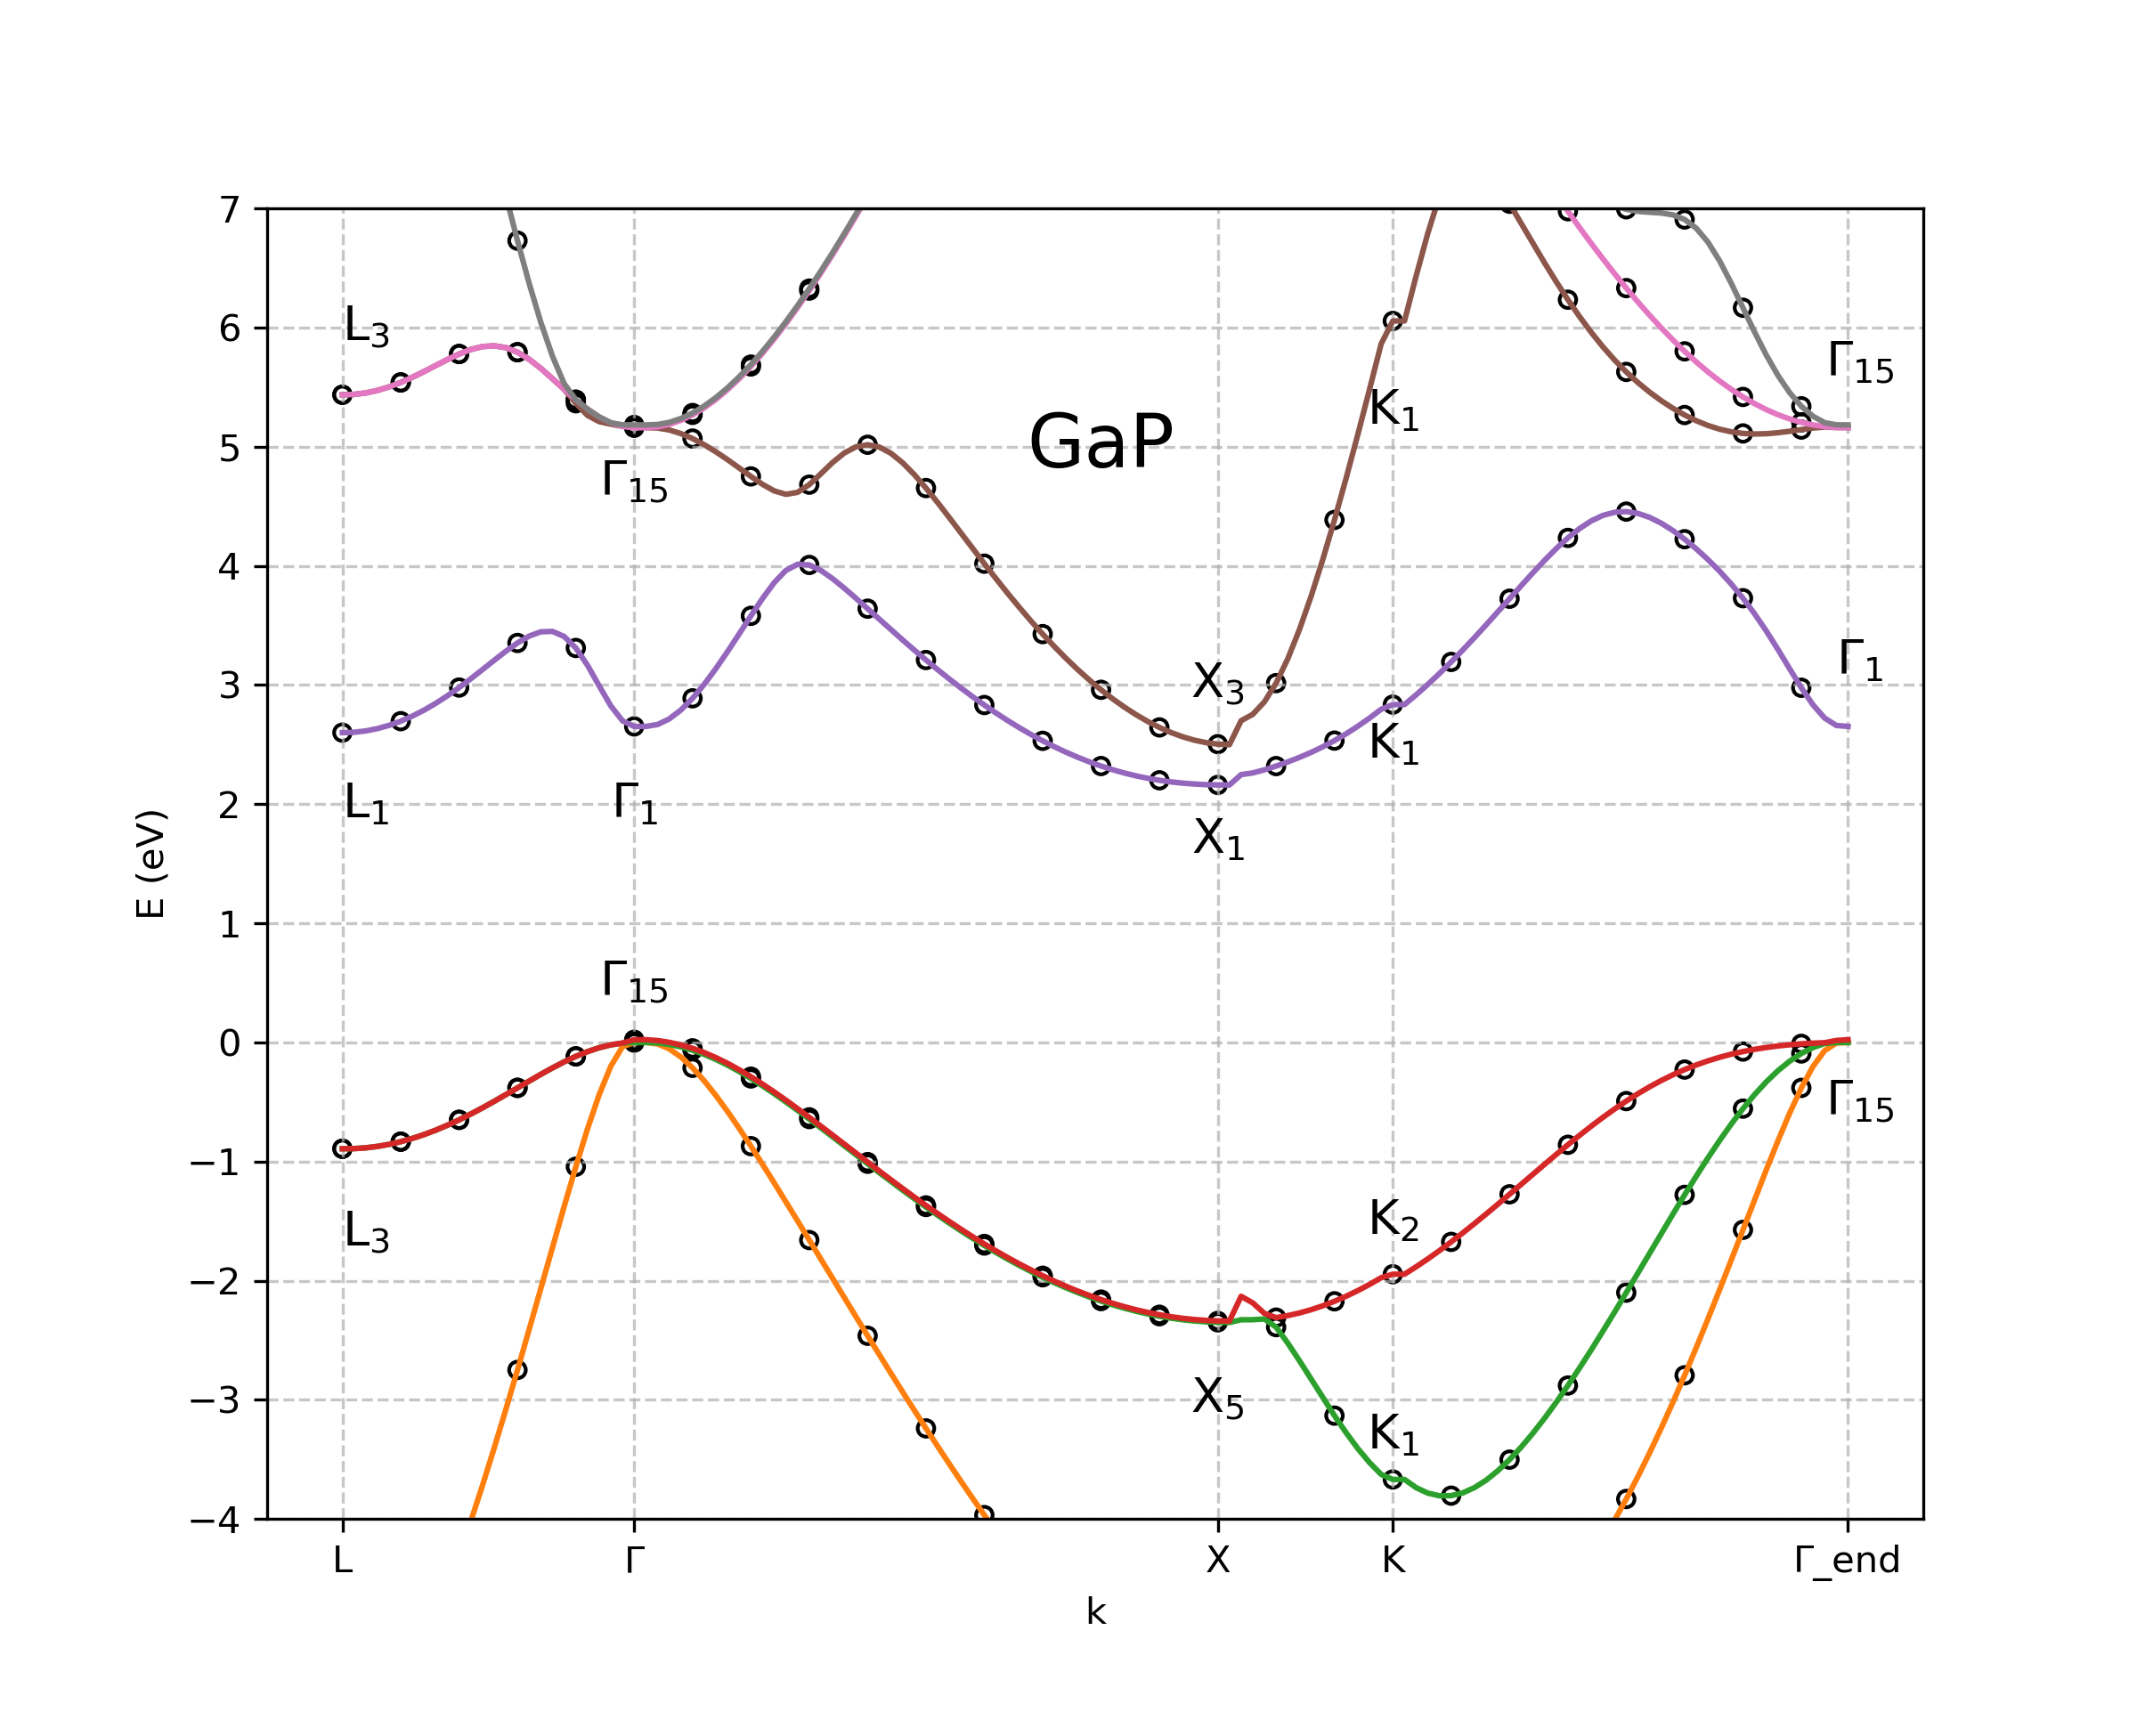
\includegraphics[width=\linewidth]{Gap.png}
    \vspace{-1cm}
    \caption{Band structure of GaP.}
    \label{fig:GaP}

    \centering
    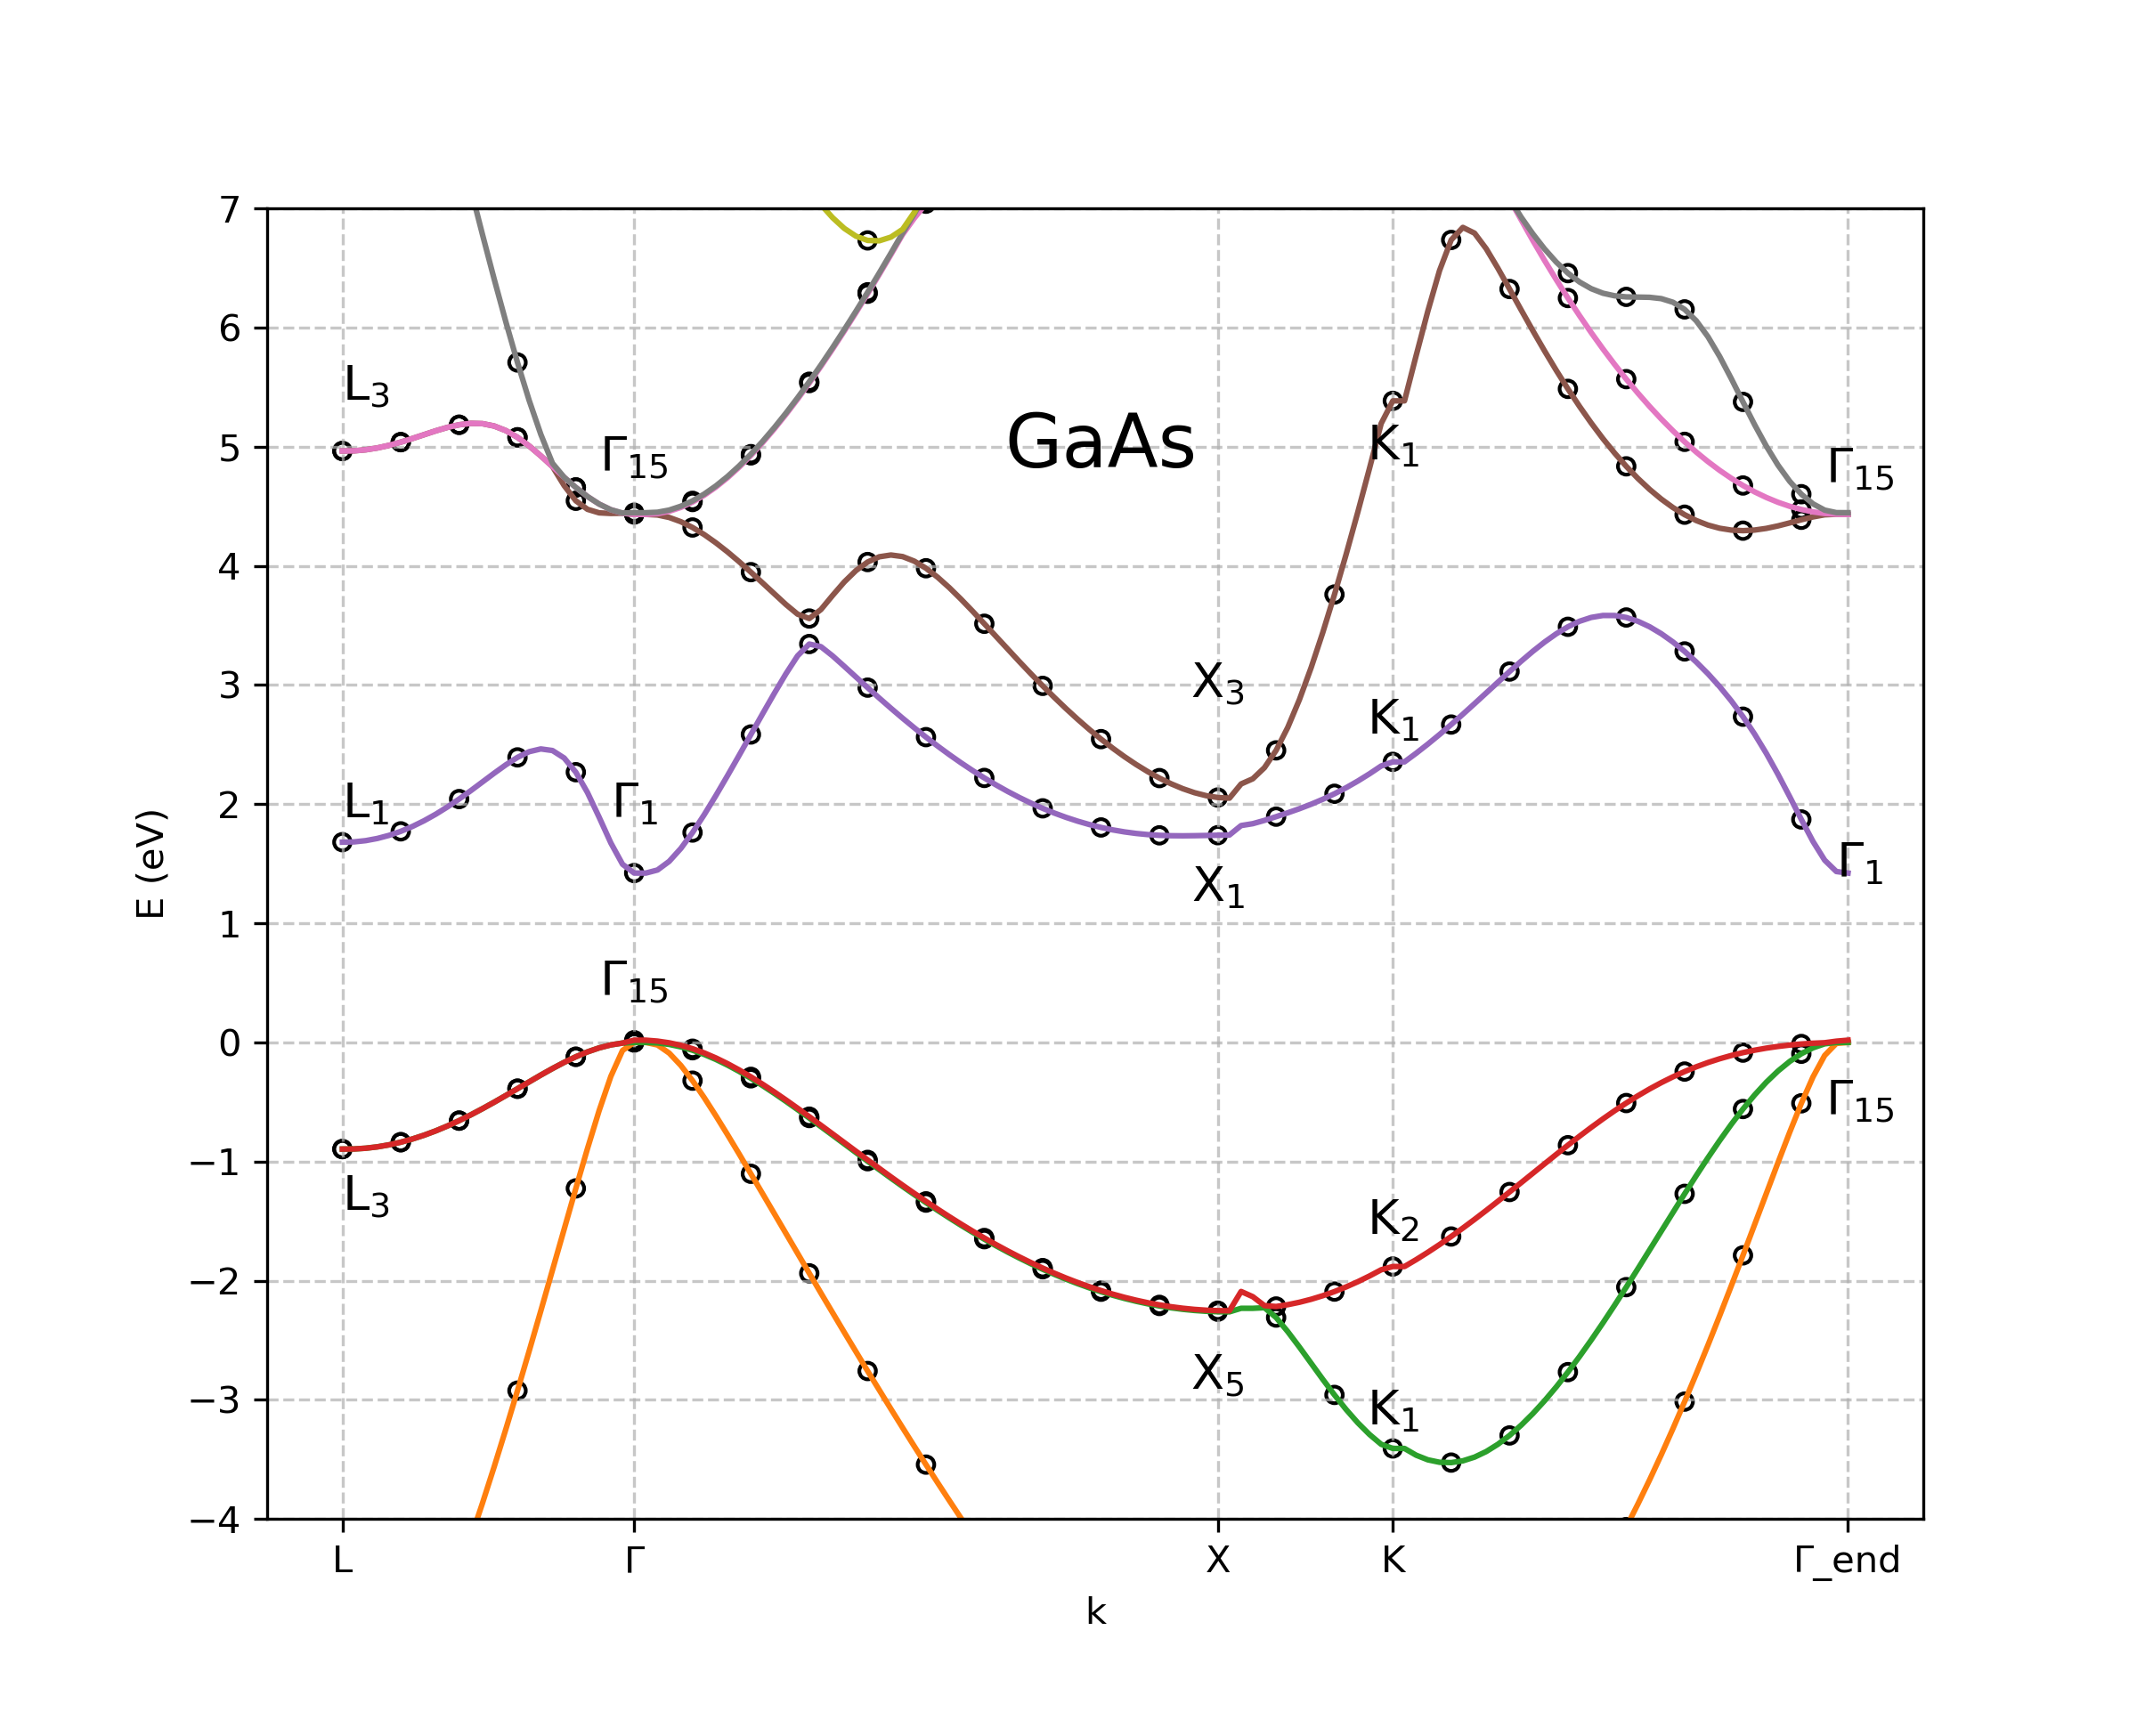
\includegraphics[width=\linewidth]{GaAs.png}
    \vspace{-1cm}
    \caption{Band structure of GaAs.}
    \label{fig:GaAs}
\end{figure}

\begin{figure}[htb]
    \centering
    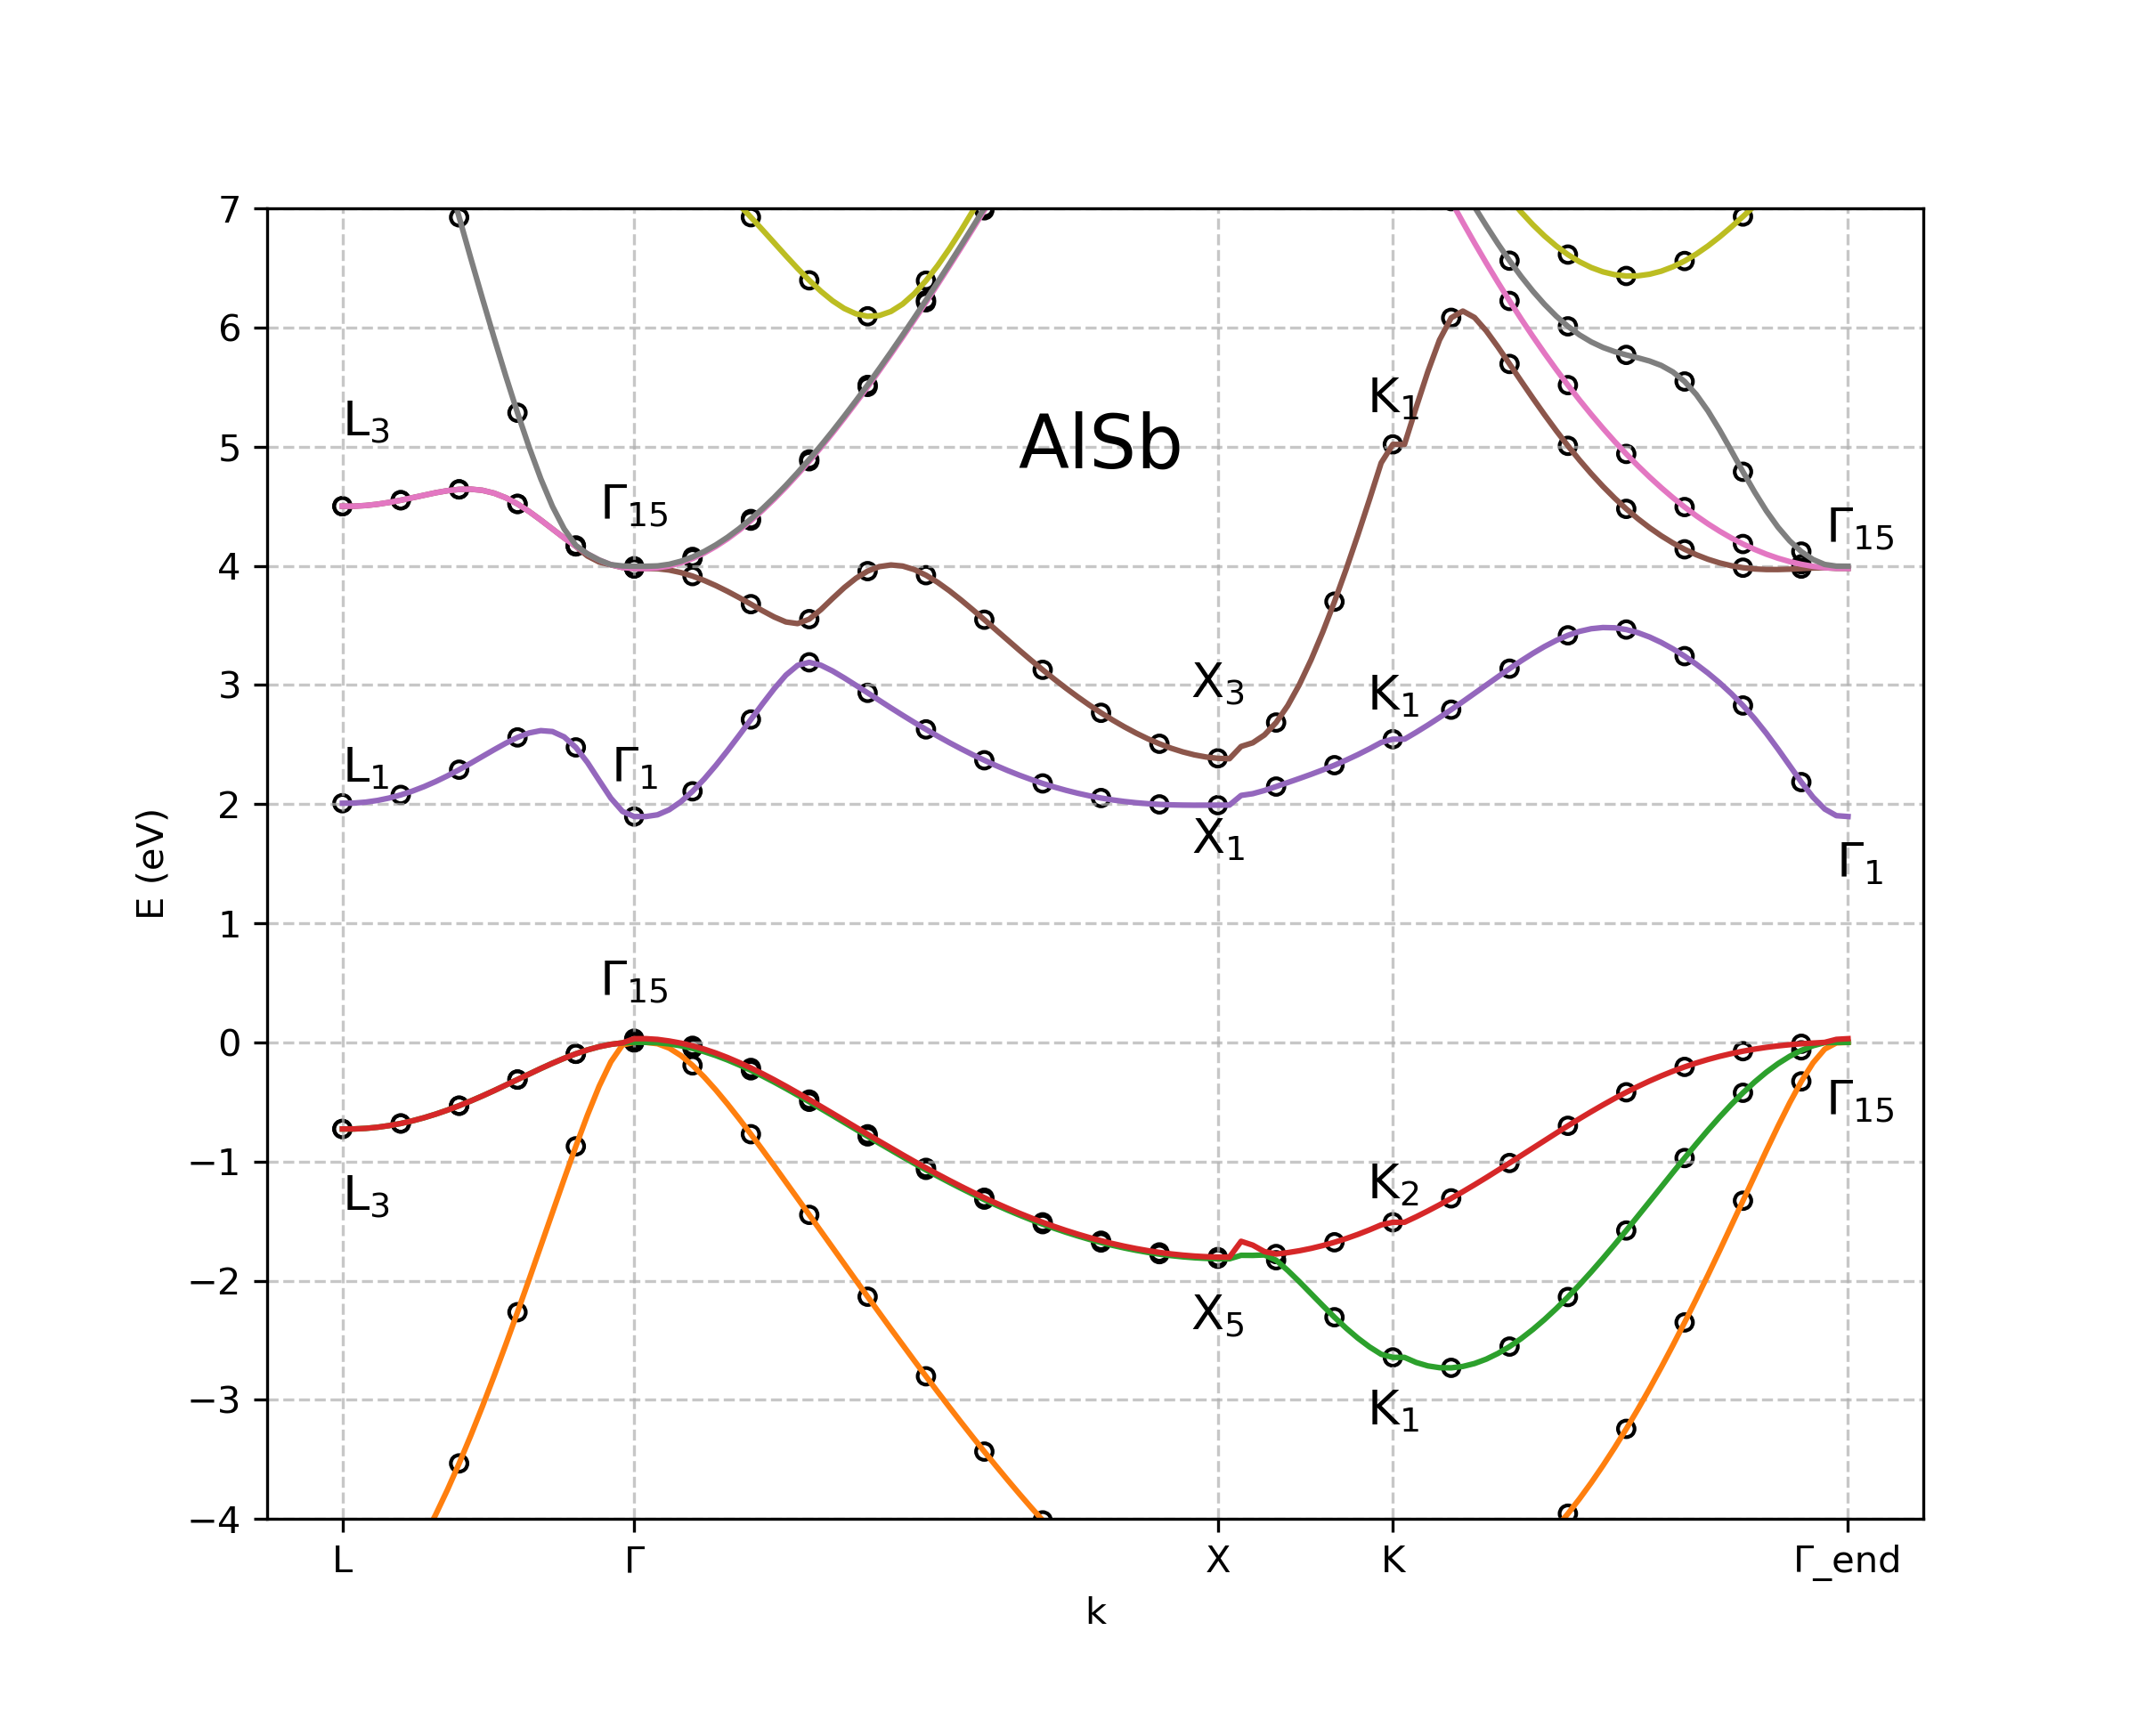
\includegraphics[width=\linewidth]{AlSb.png}
    \vspace{-1cm}
    \caption{Band structure of AlSb.}
    \label{fig:AlSb}

    \centering
    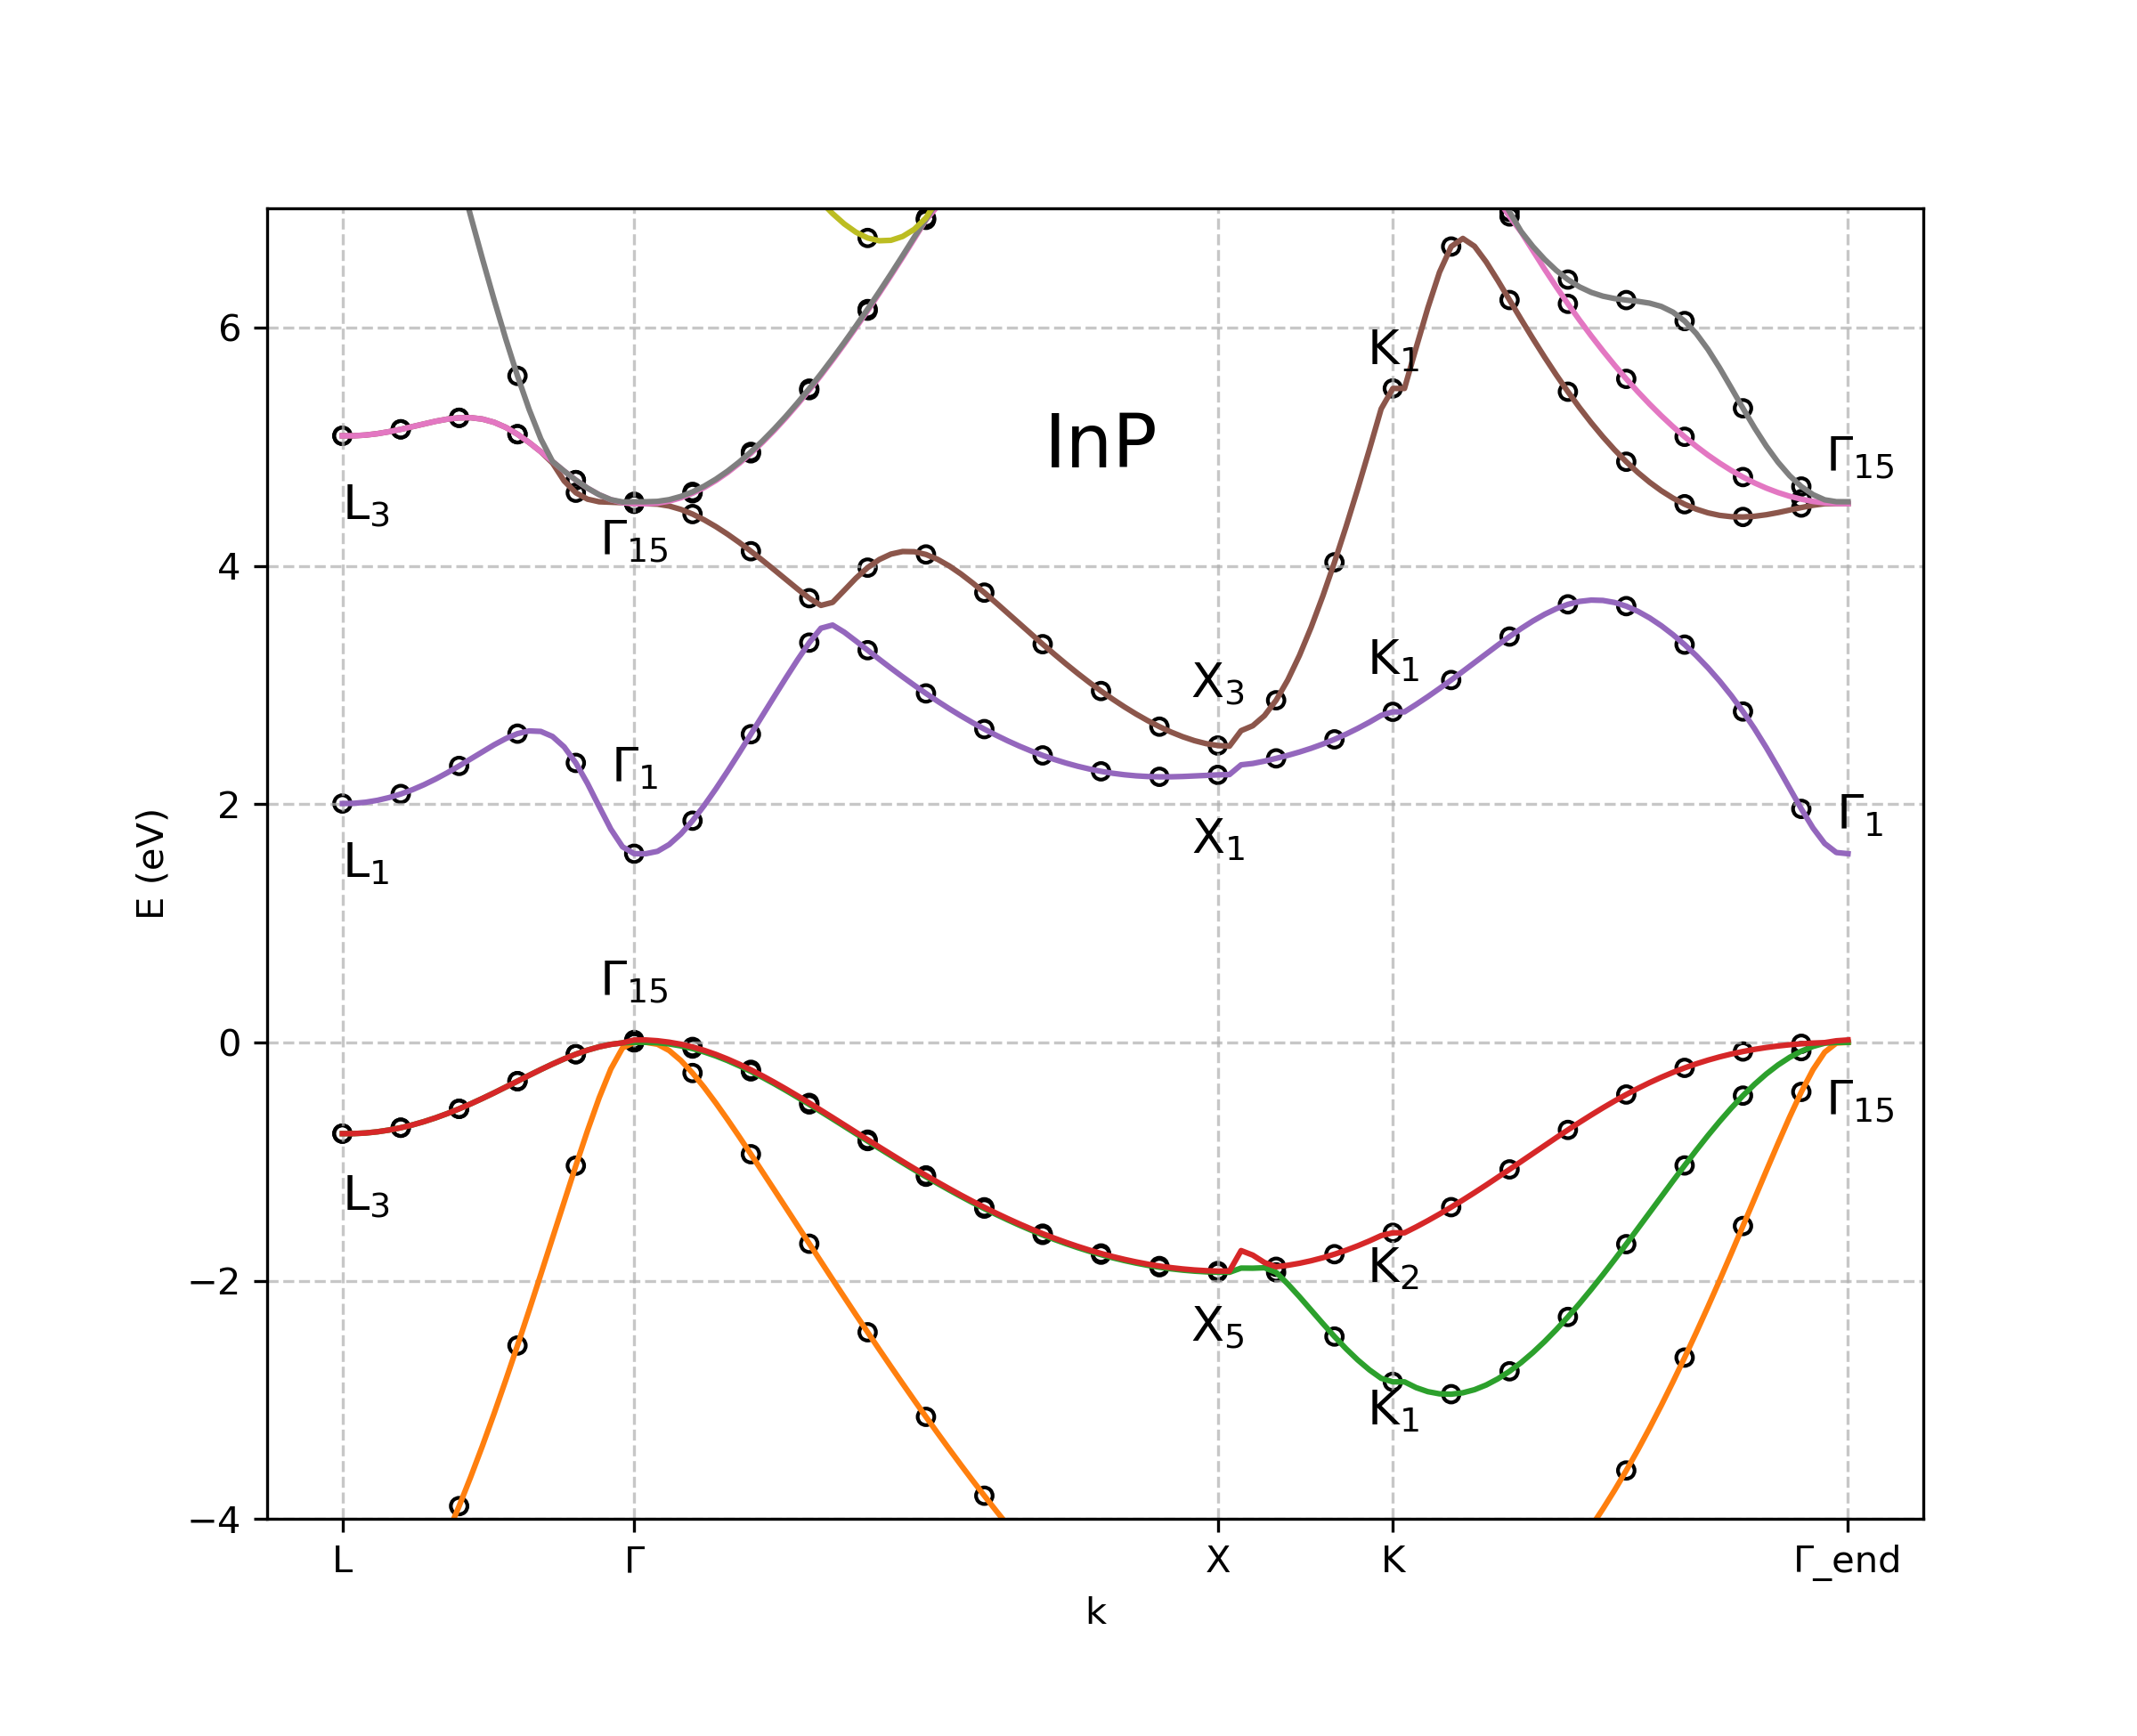
\includegraphics[width=\linewidth]{InP.png}
    \vspace{-1cm}

    \caption{Band structure of InP.}
    \label{fig:InP}

    \centering
    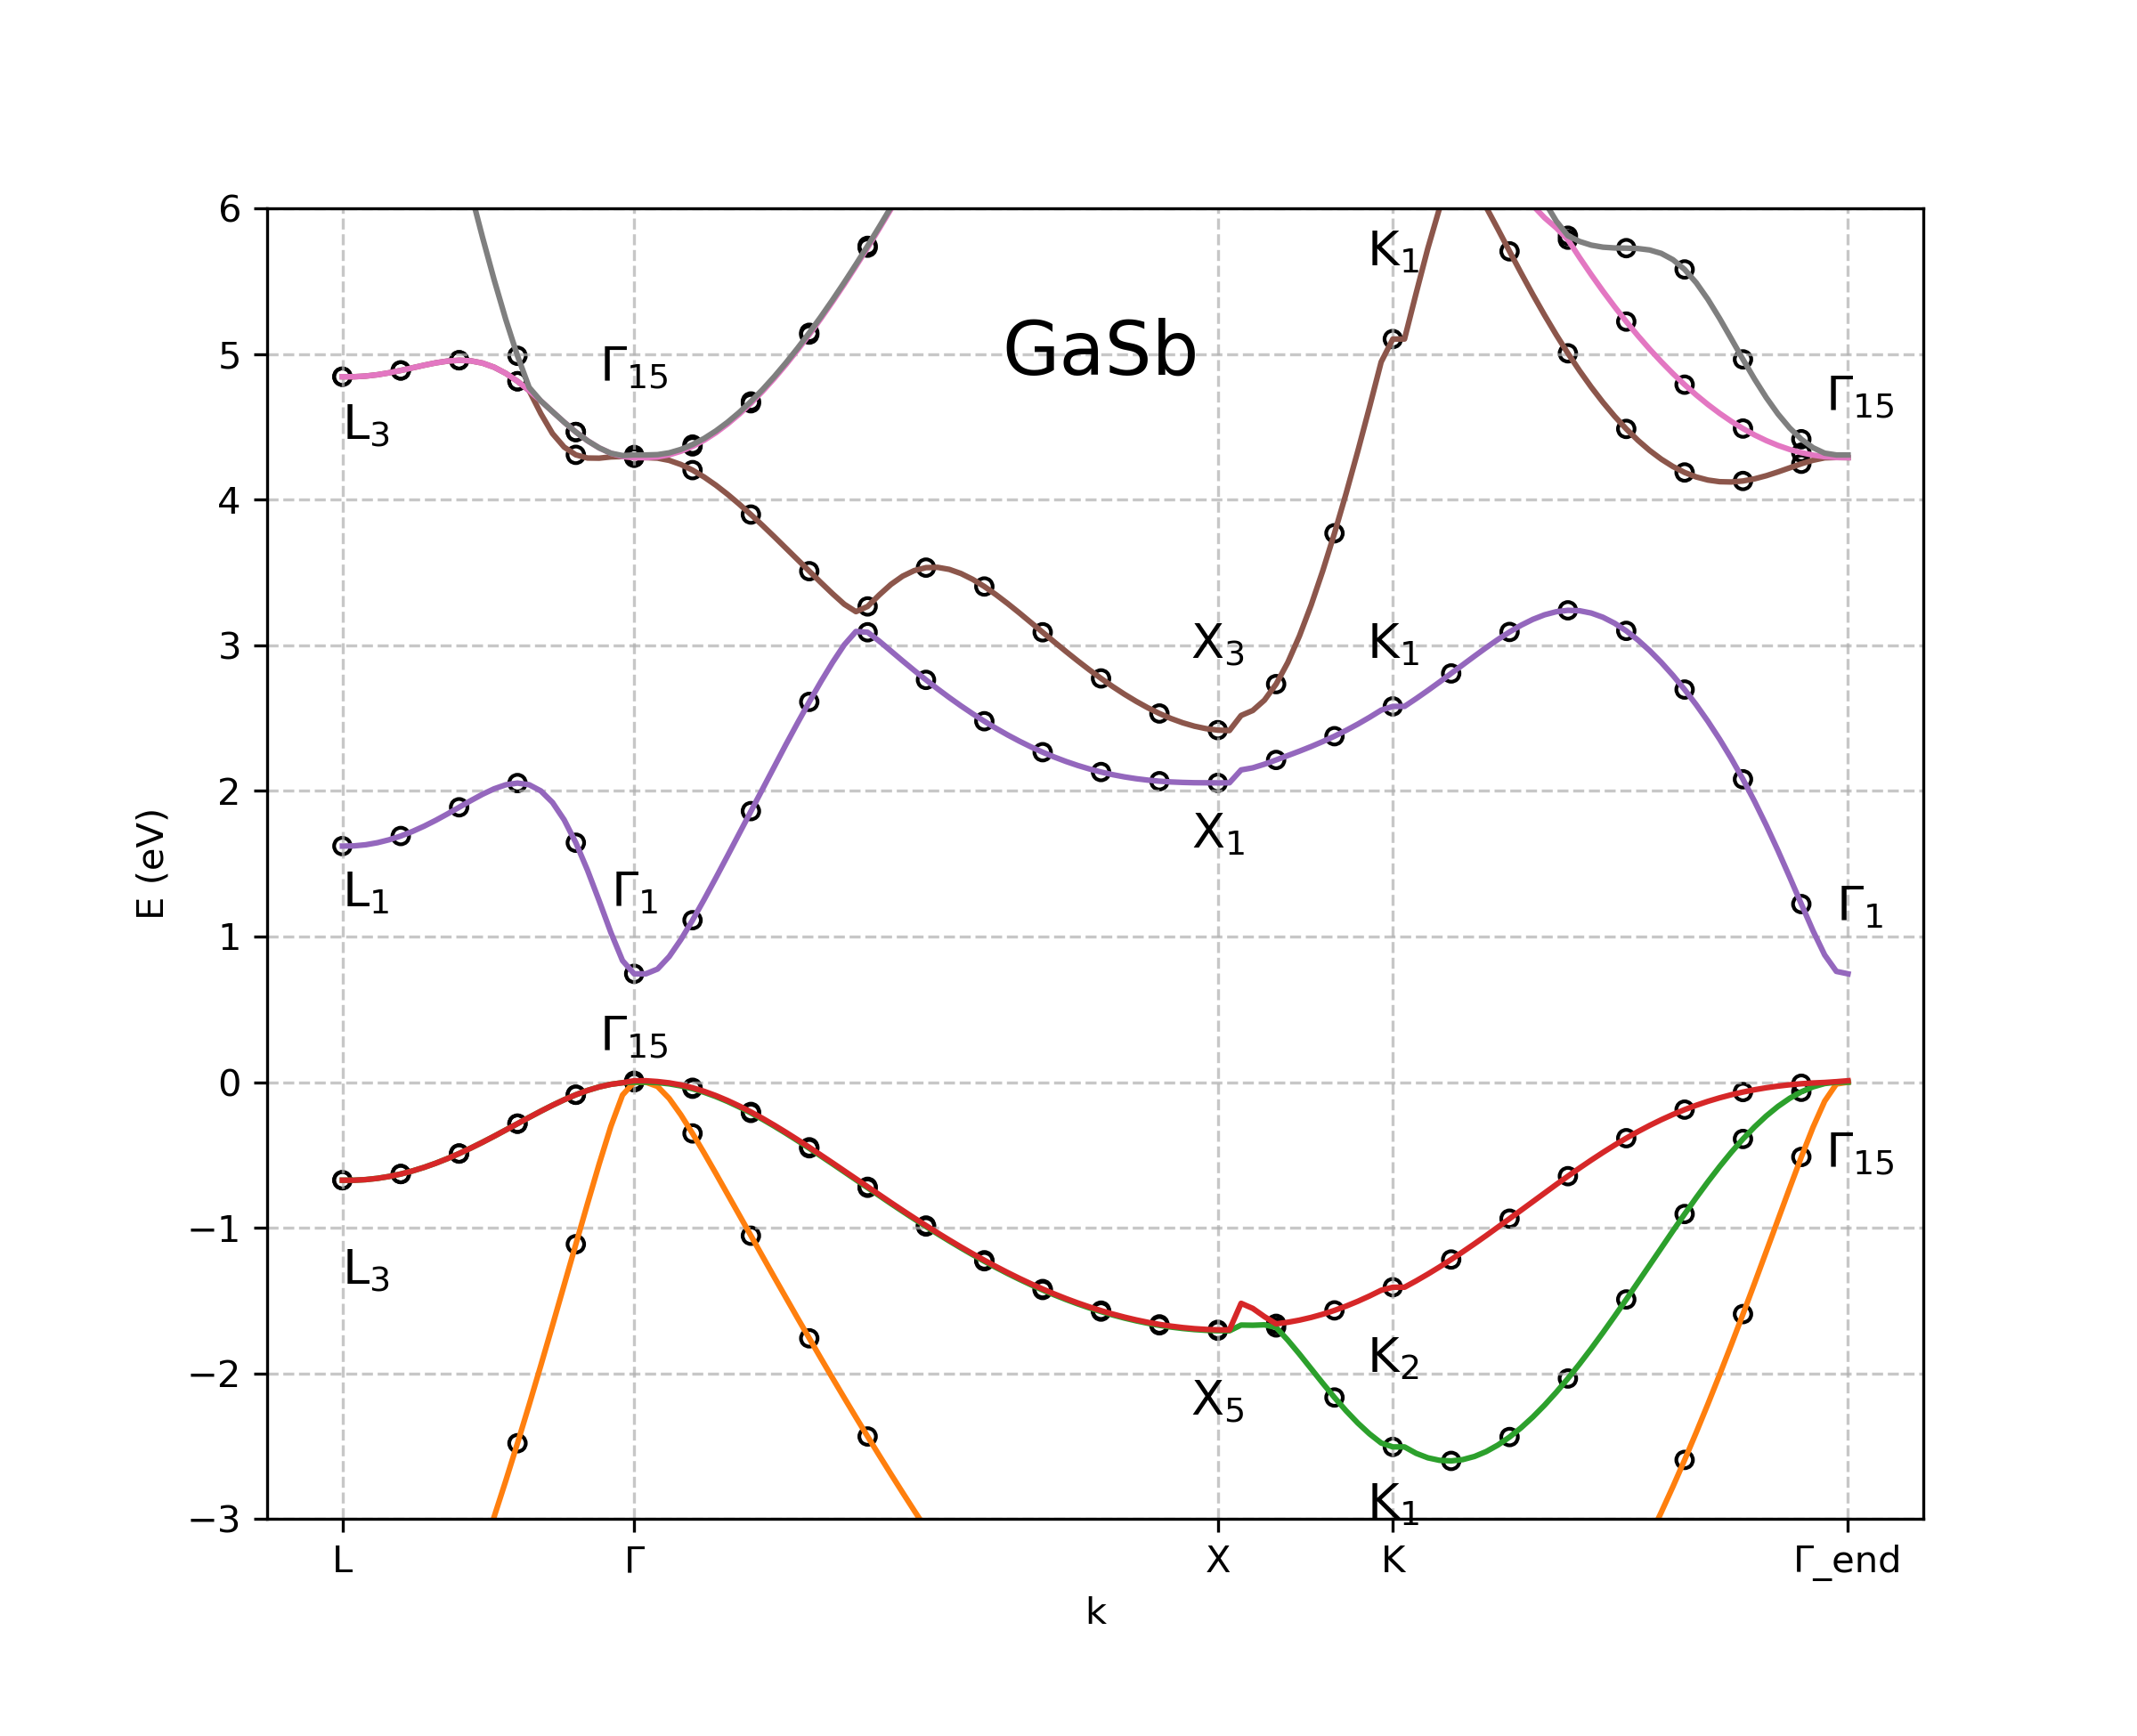
\includegraphics[width=\linewidth]{GaSb.png}
    \vspace{-1cm}
    \caption{Band structure of GaSb.}
    \label{fig:GaSb}
\end{figure}

\begin{figure}[htb]
    \centering
    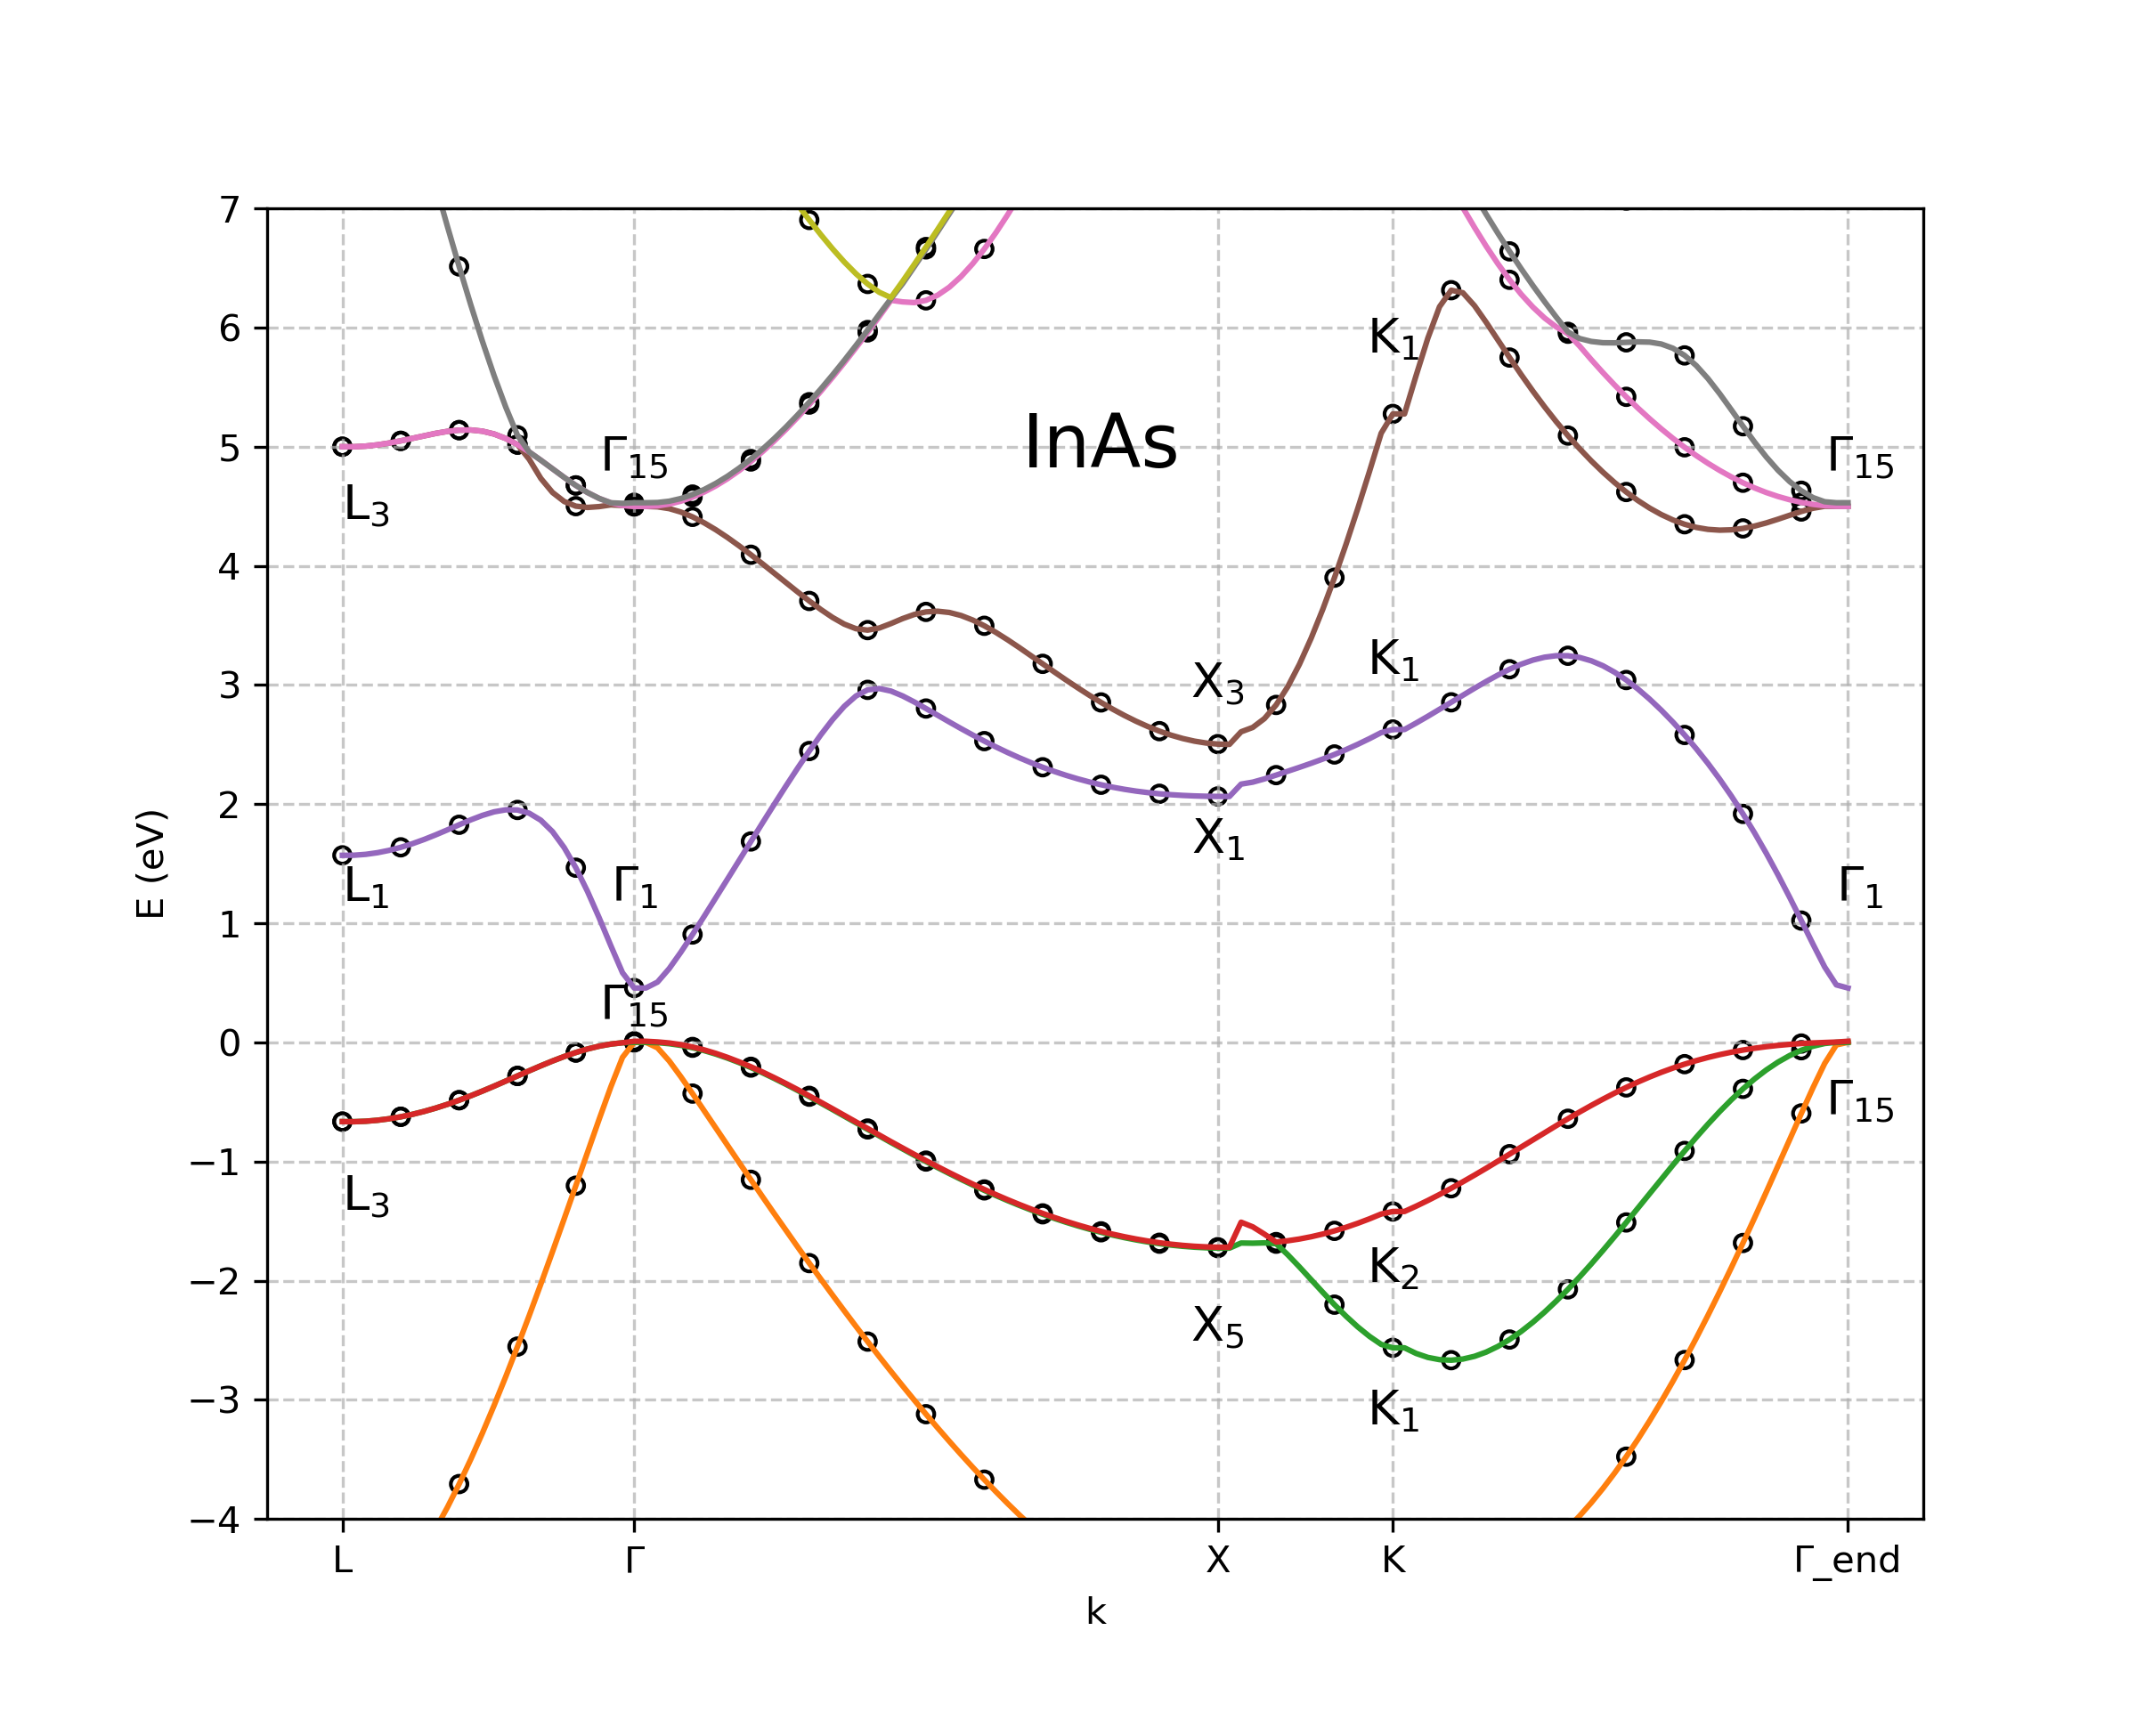
\includegraphics[width=\linewidth]{InAs.png}
    \vspace{-1cm}
    \caption{Band structure of InAs.}
    \label{fig:InAs}

    \centering
    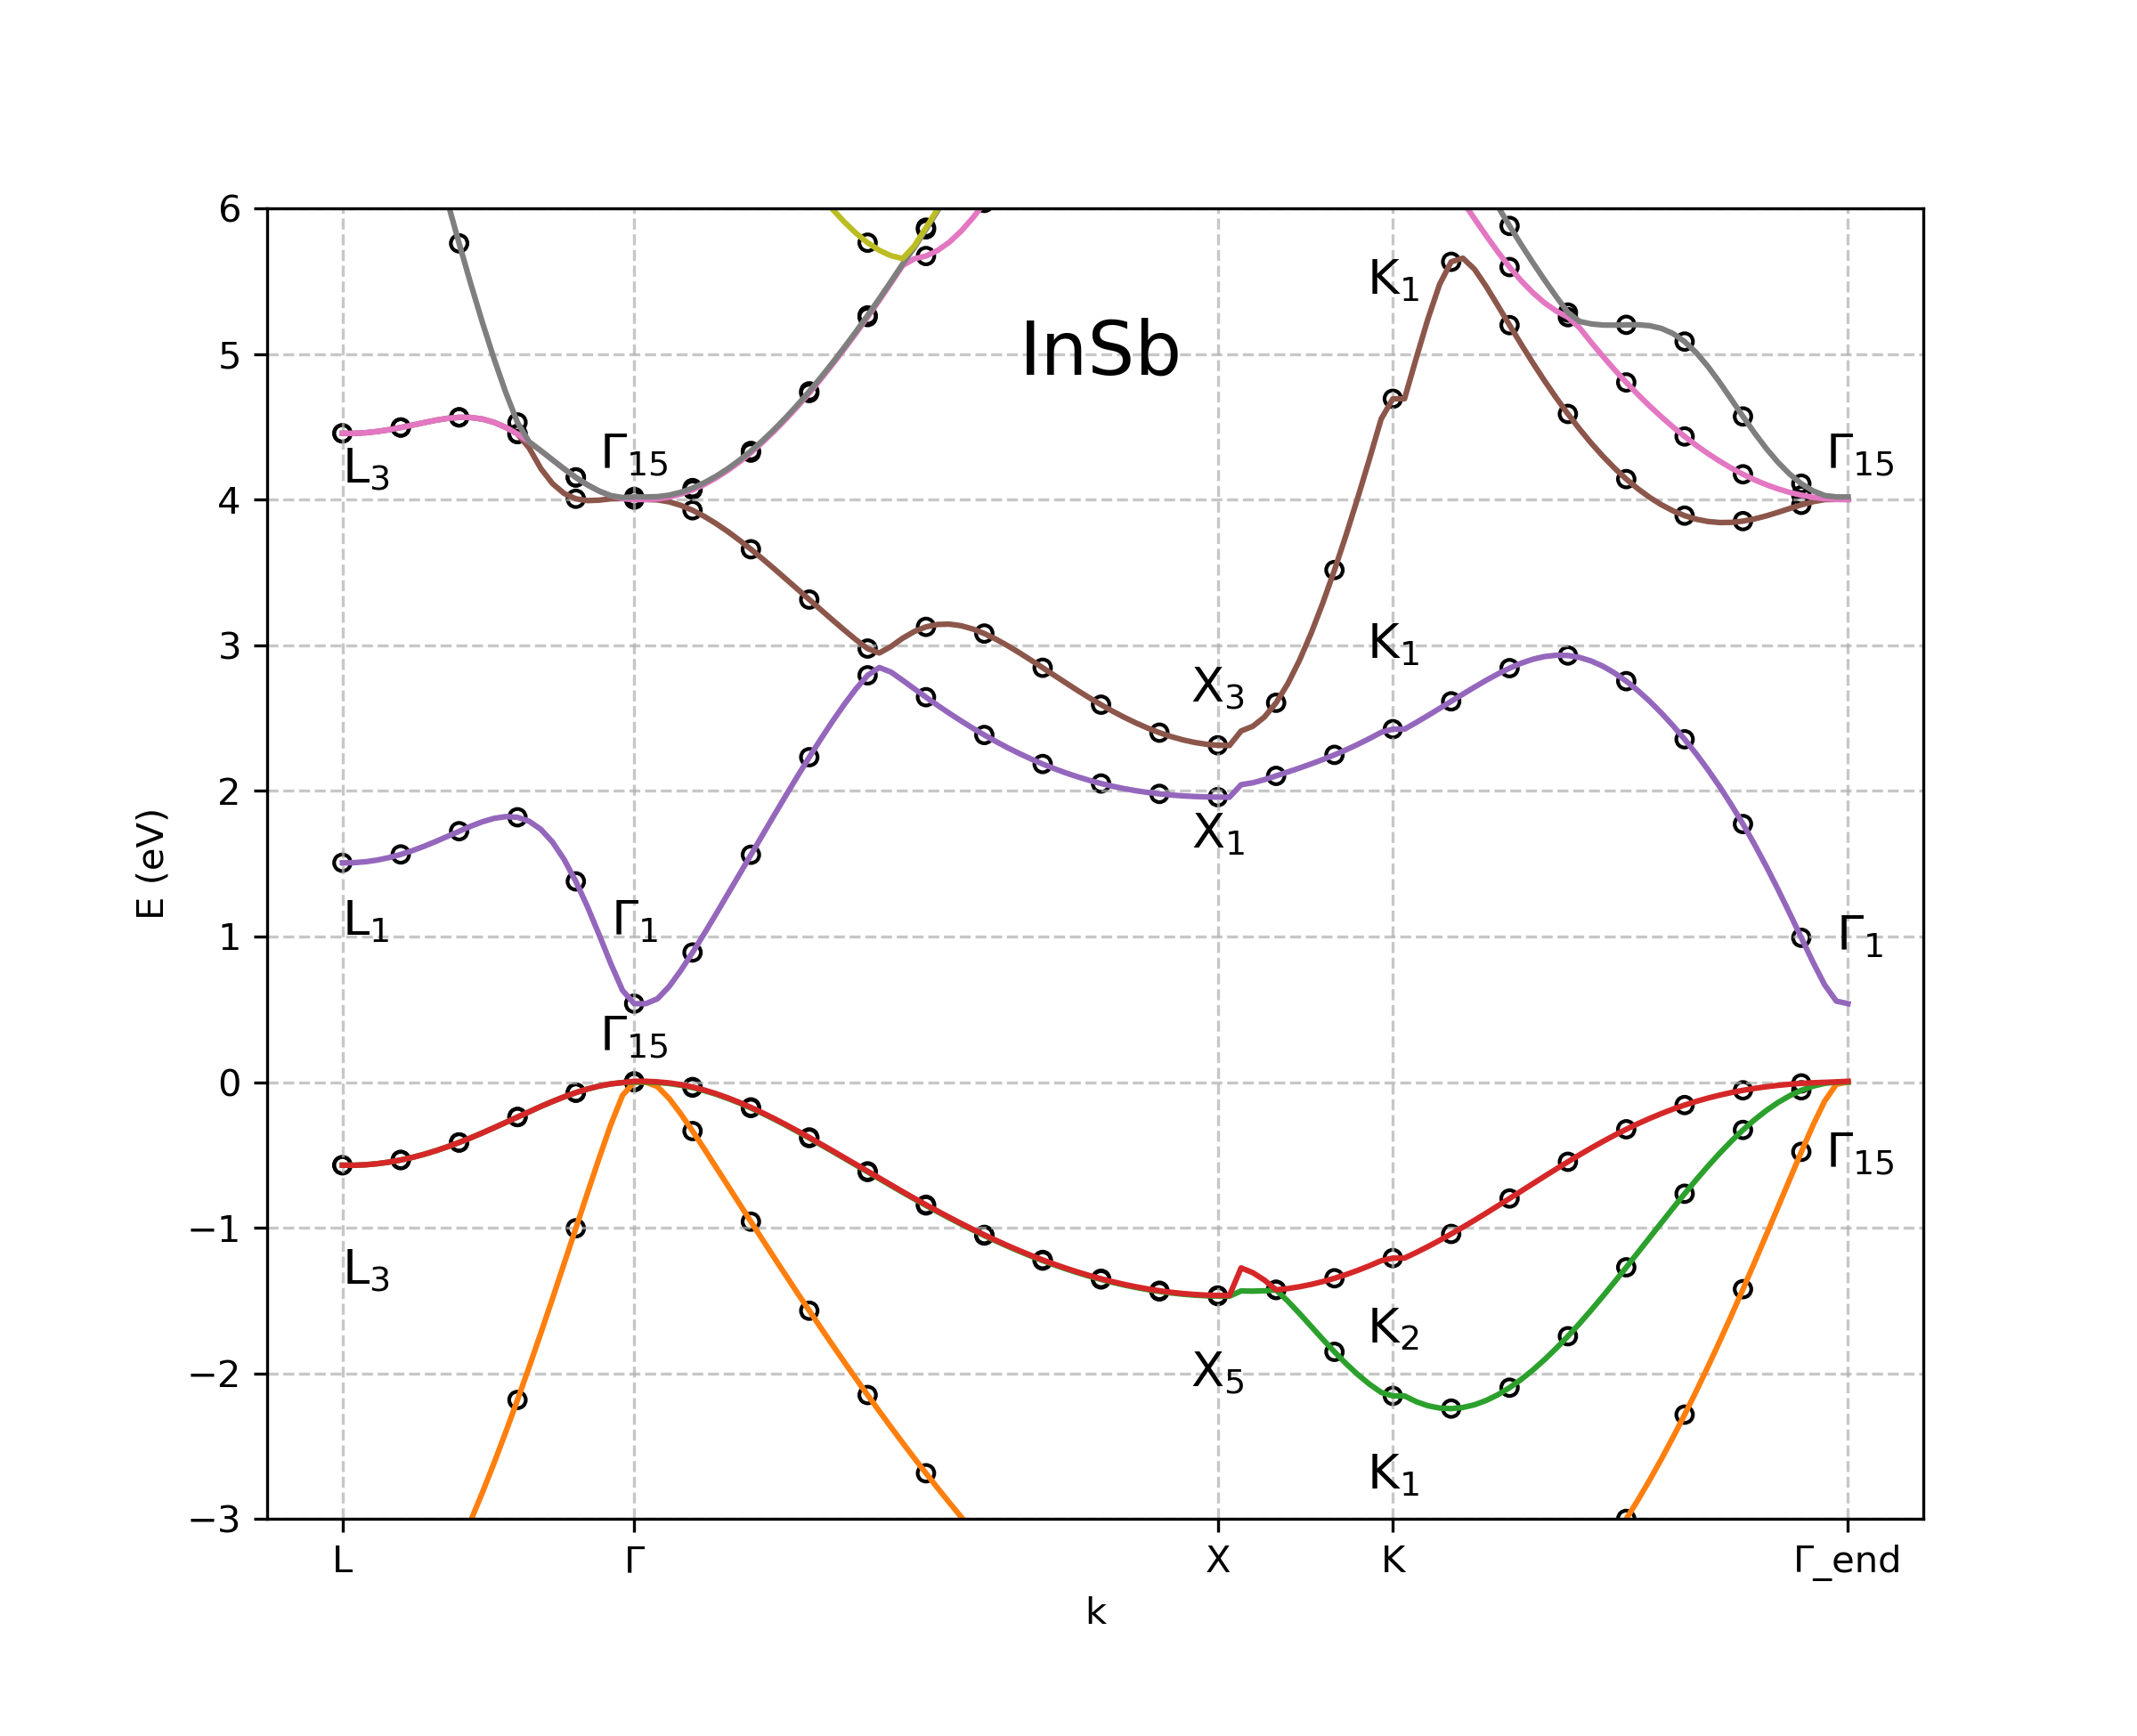
\includegraphics[width=\linewidth]{InSb.png}
    \vspace{-1cm}
    \caption{Band structure of InSb.}
    \label{fig:InSb}

    \centering
    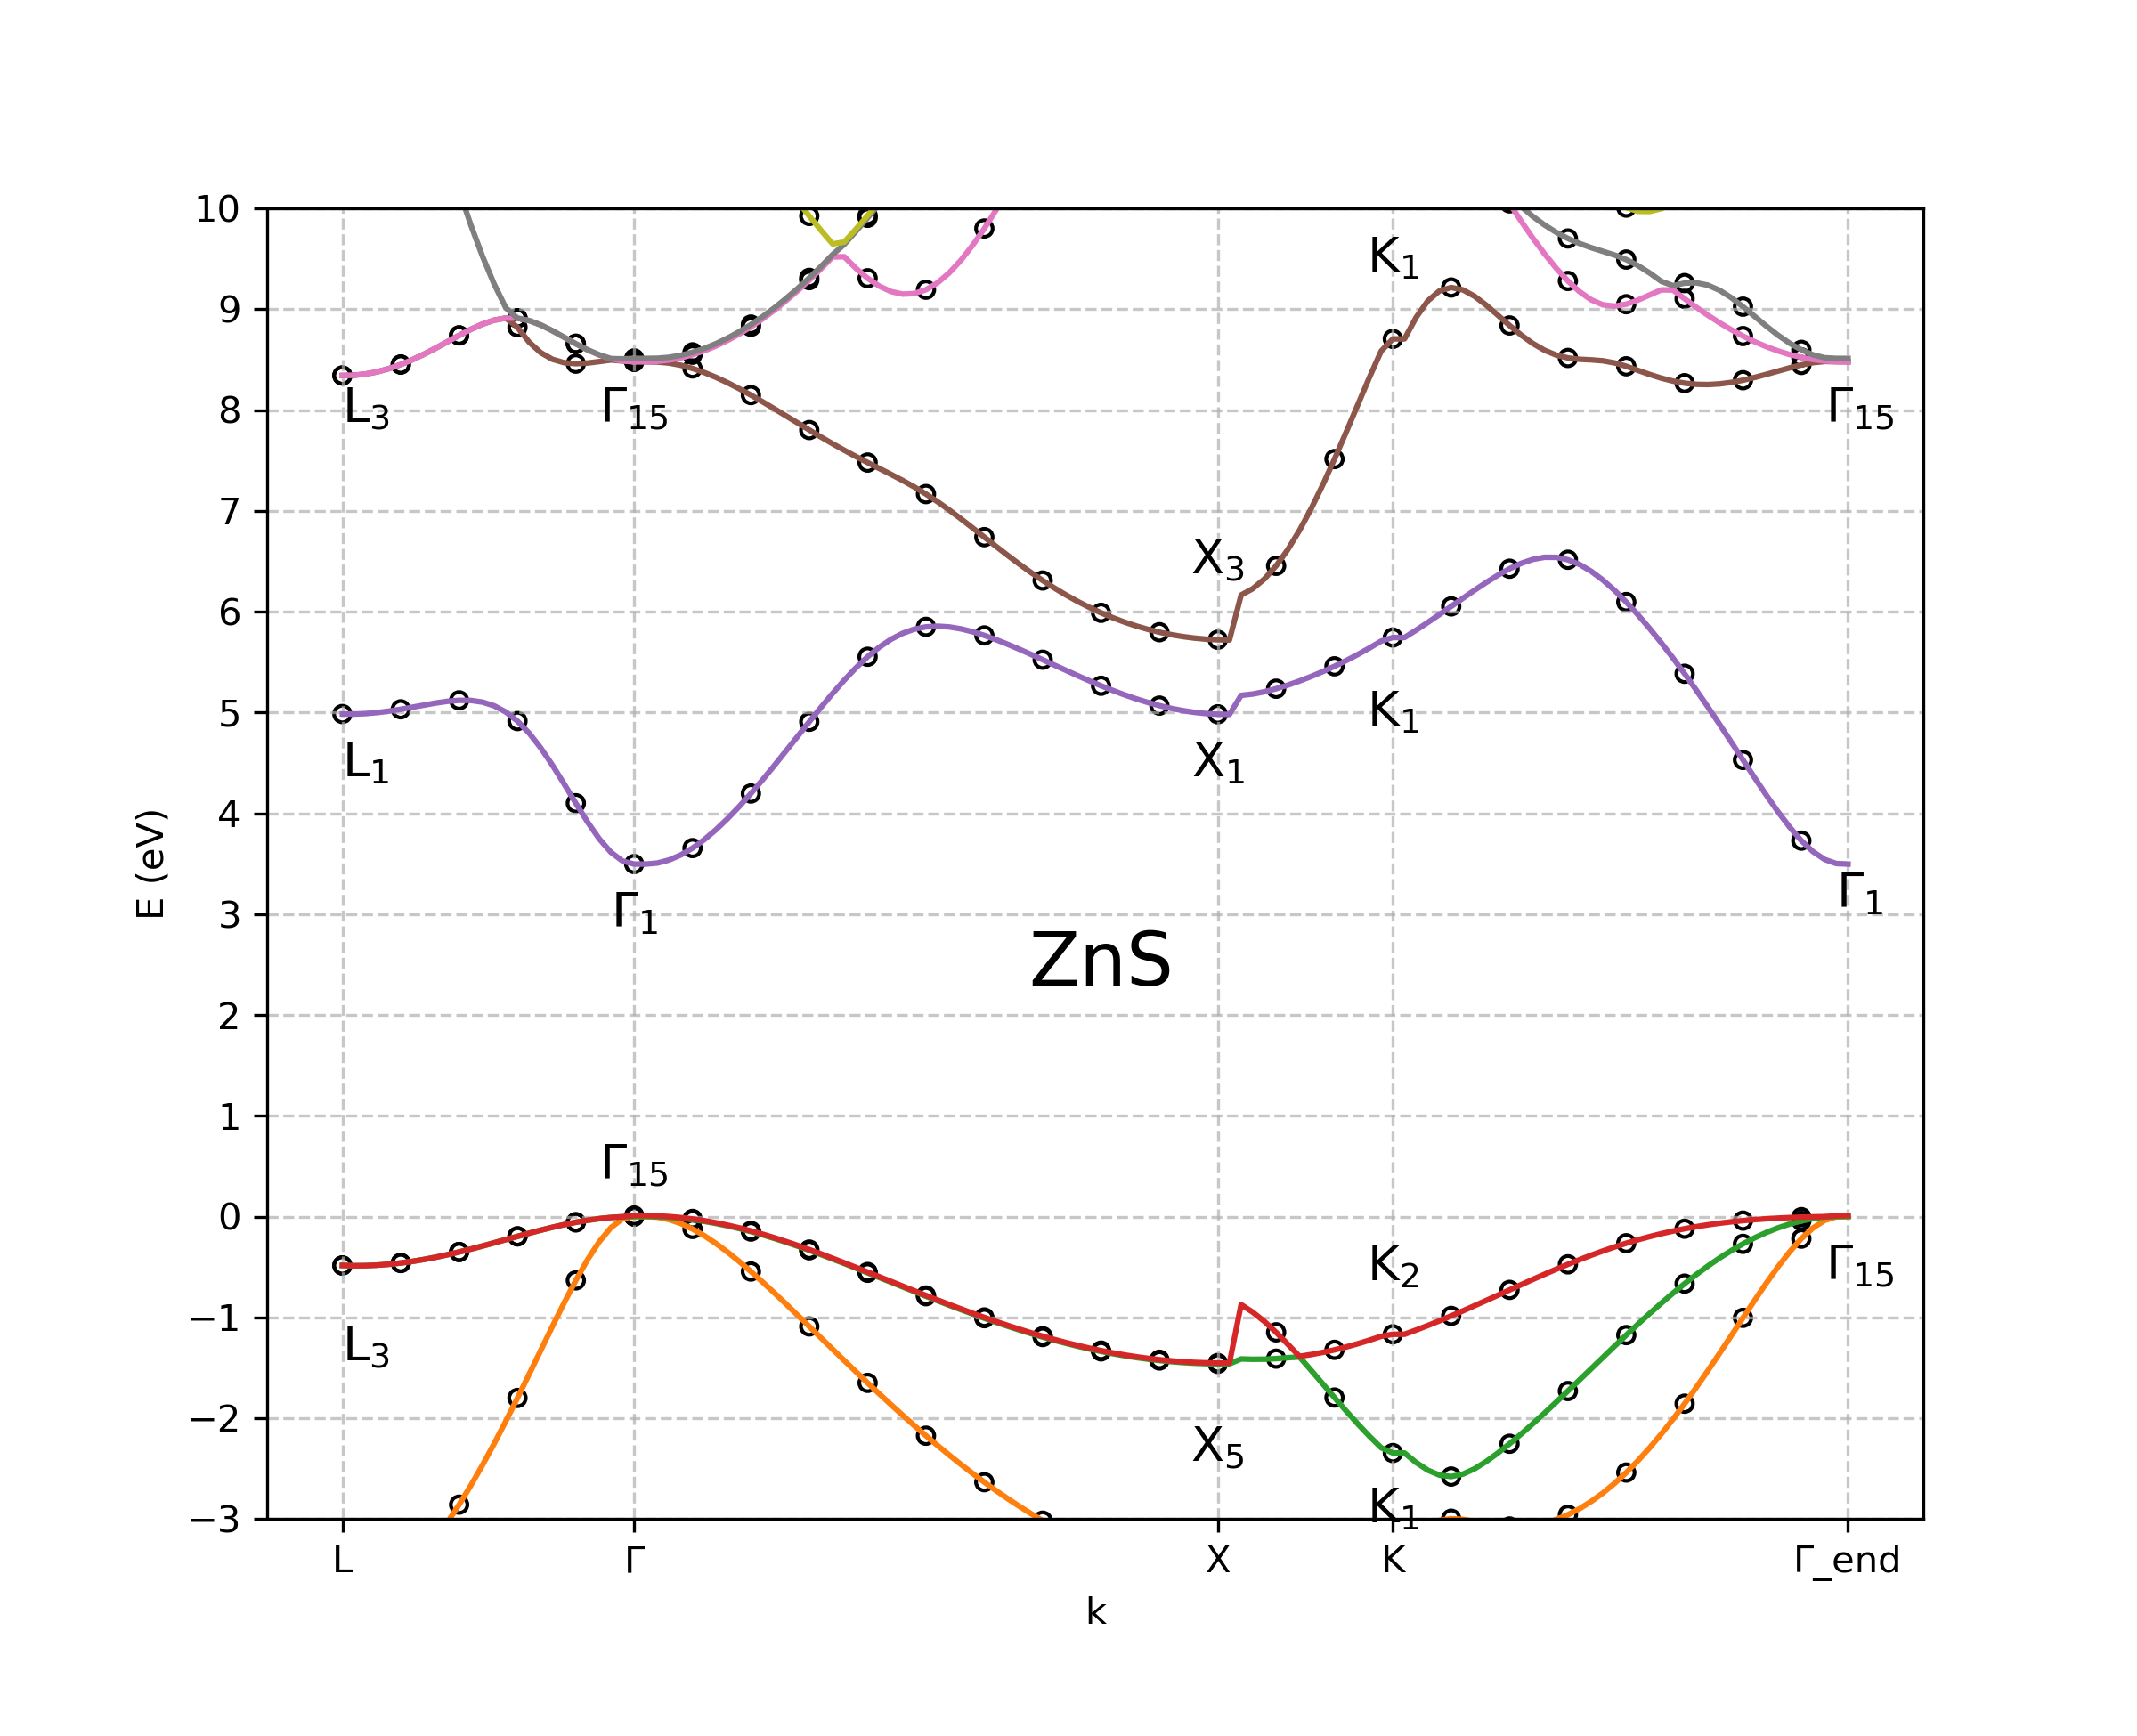
\includegraphics[width=\linewidth]{ZnS.png}
    \vspace{-1cm}
    \caption{Band structure of ZnS.}
    \label{fig:ZnS}
\end{figure}

\begin{figure}[htb]
    \centering
    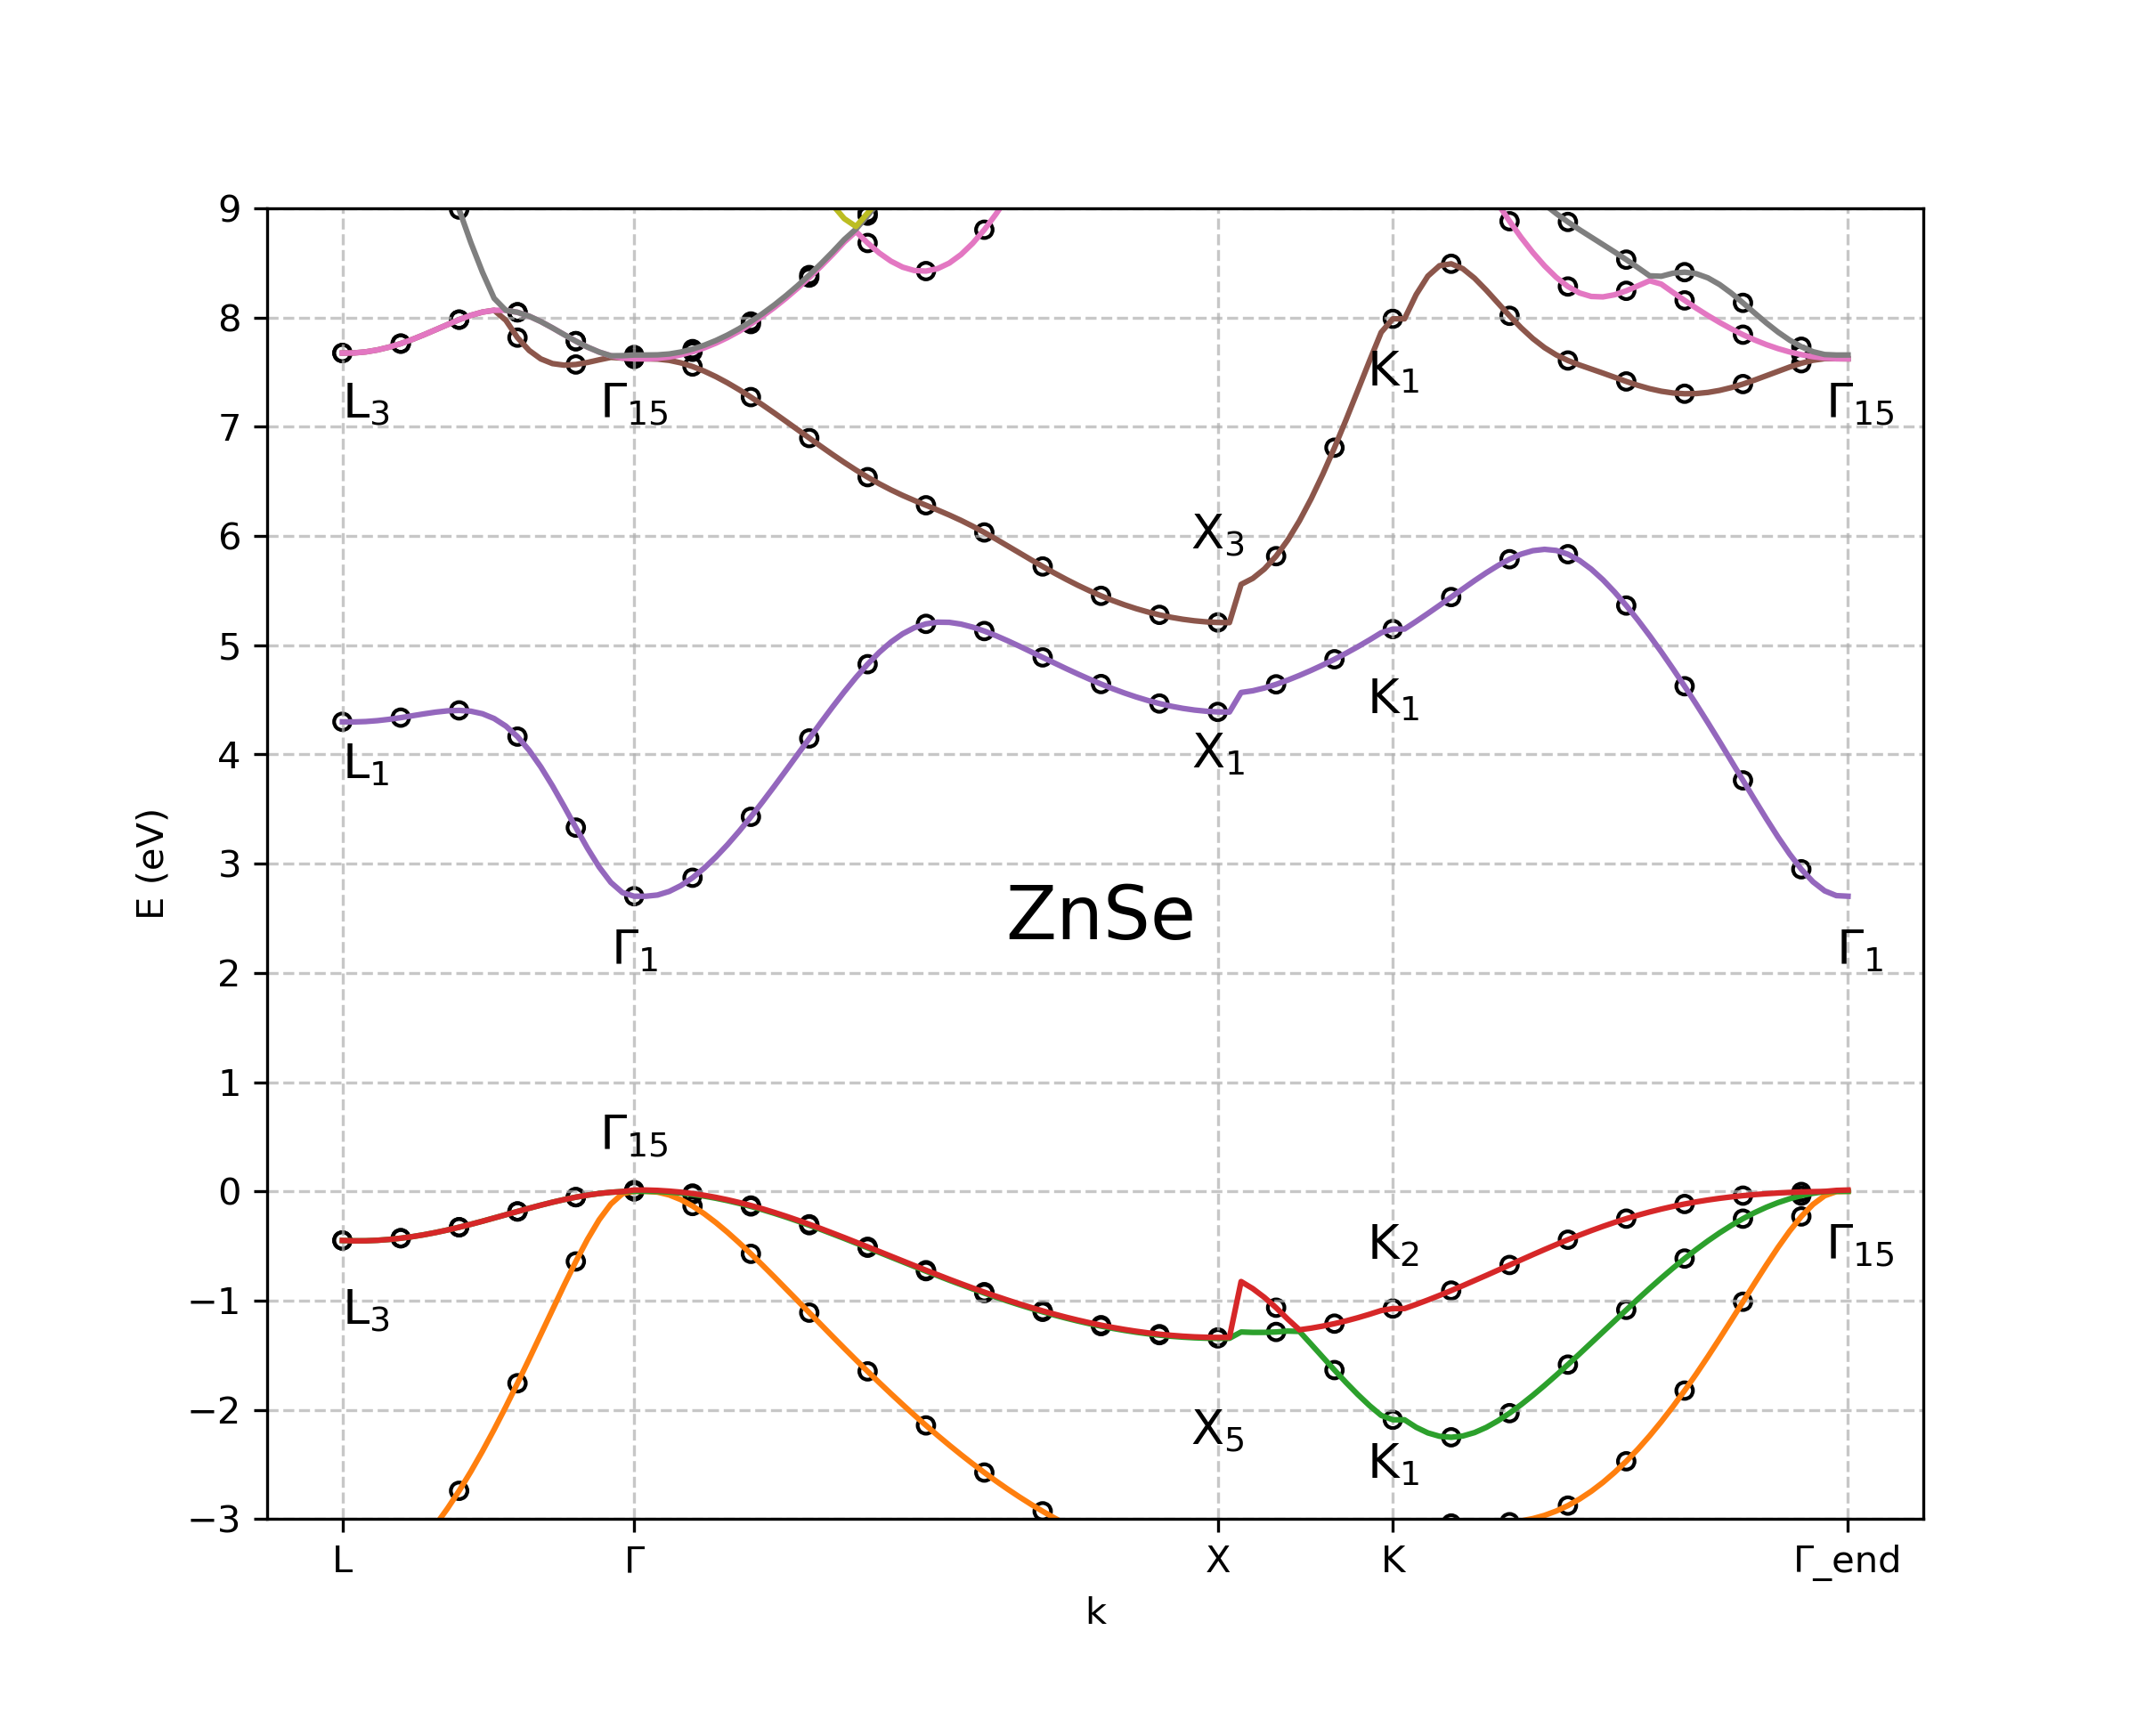
\includegraphics[width=\linewidth]{ZnSe.png}
    \vspace{-1cm}
    \caption{Band structure of ZnSe.}
    \label{fig:ZnSe}

    \centering
    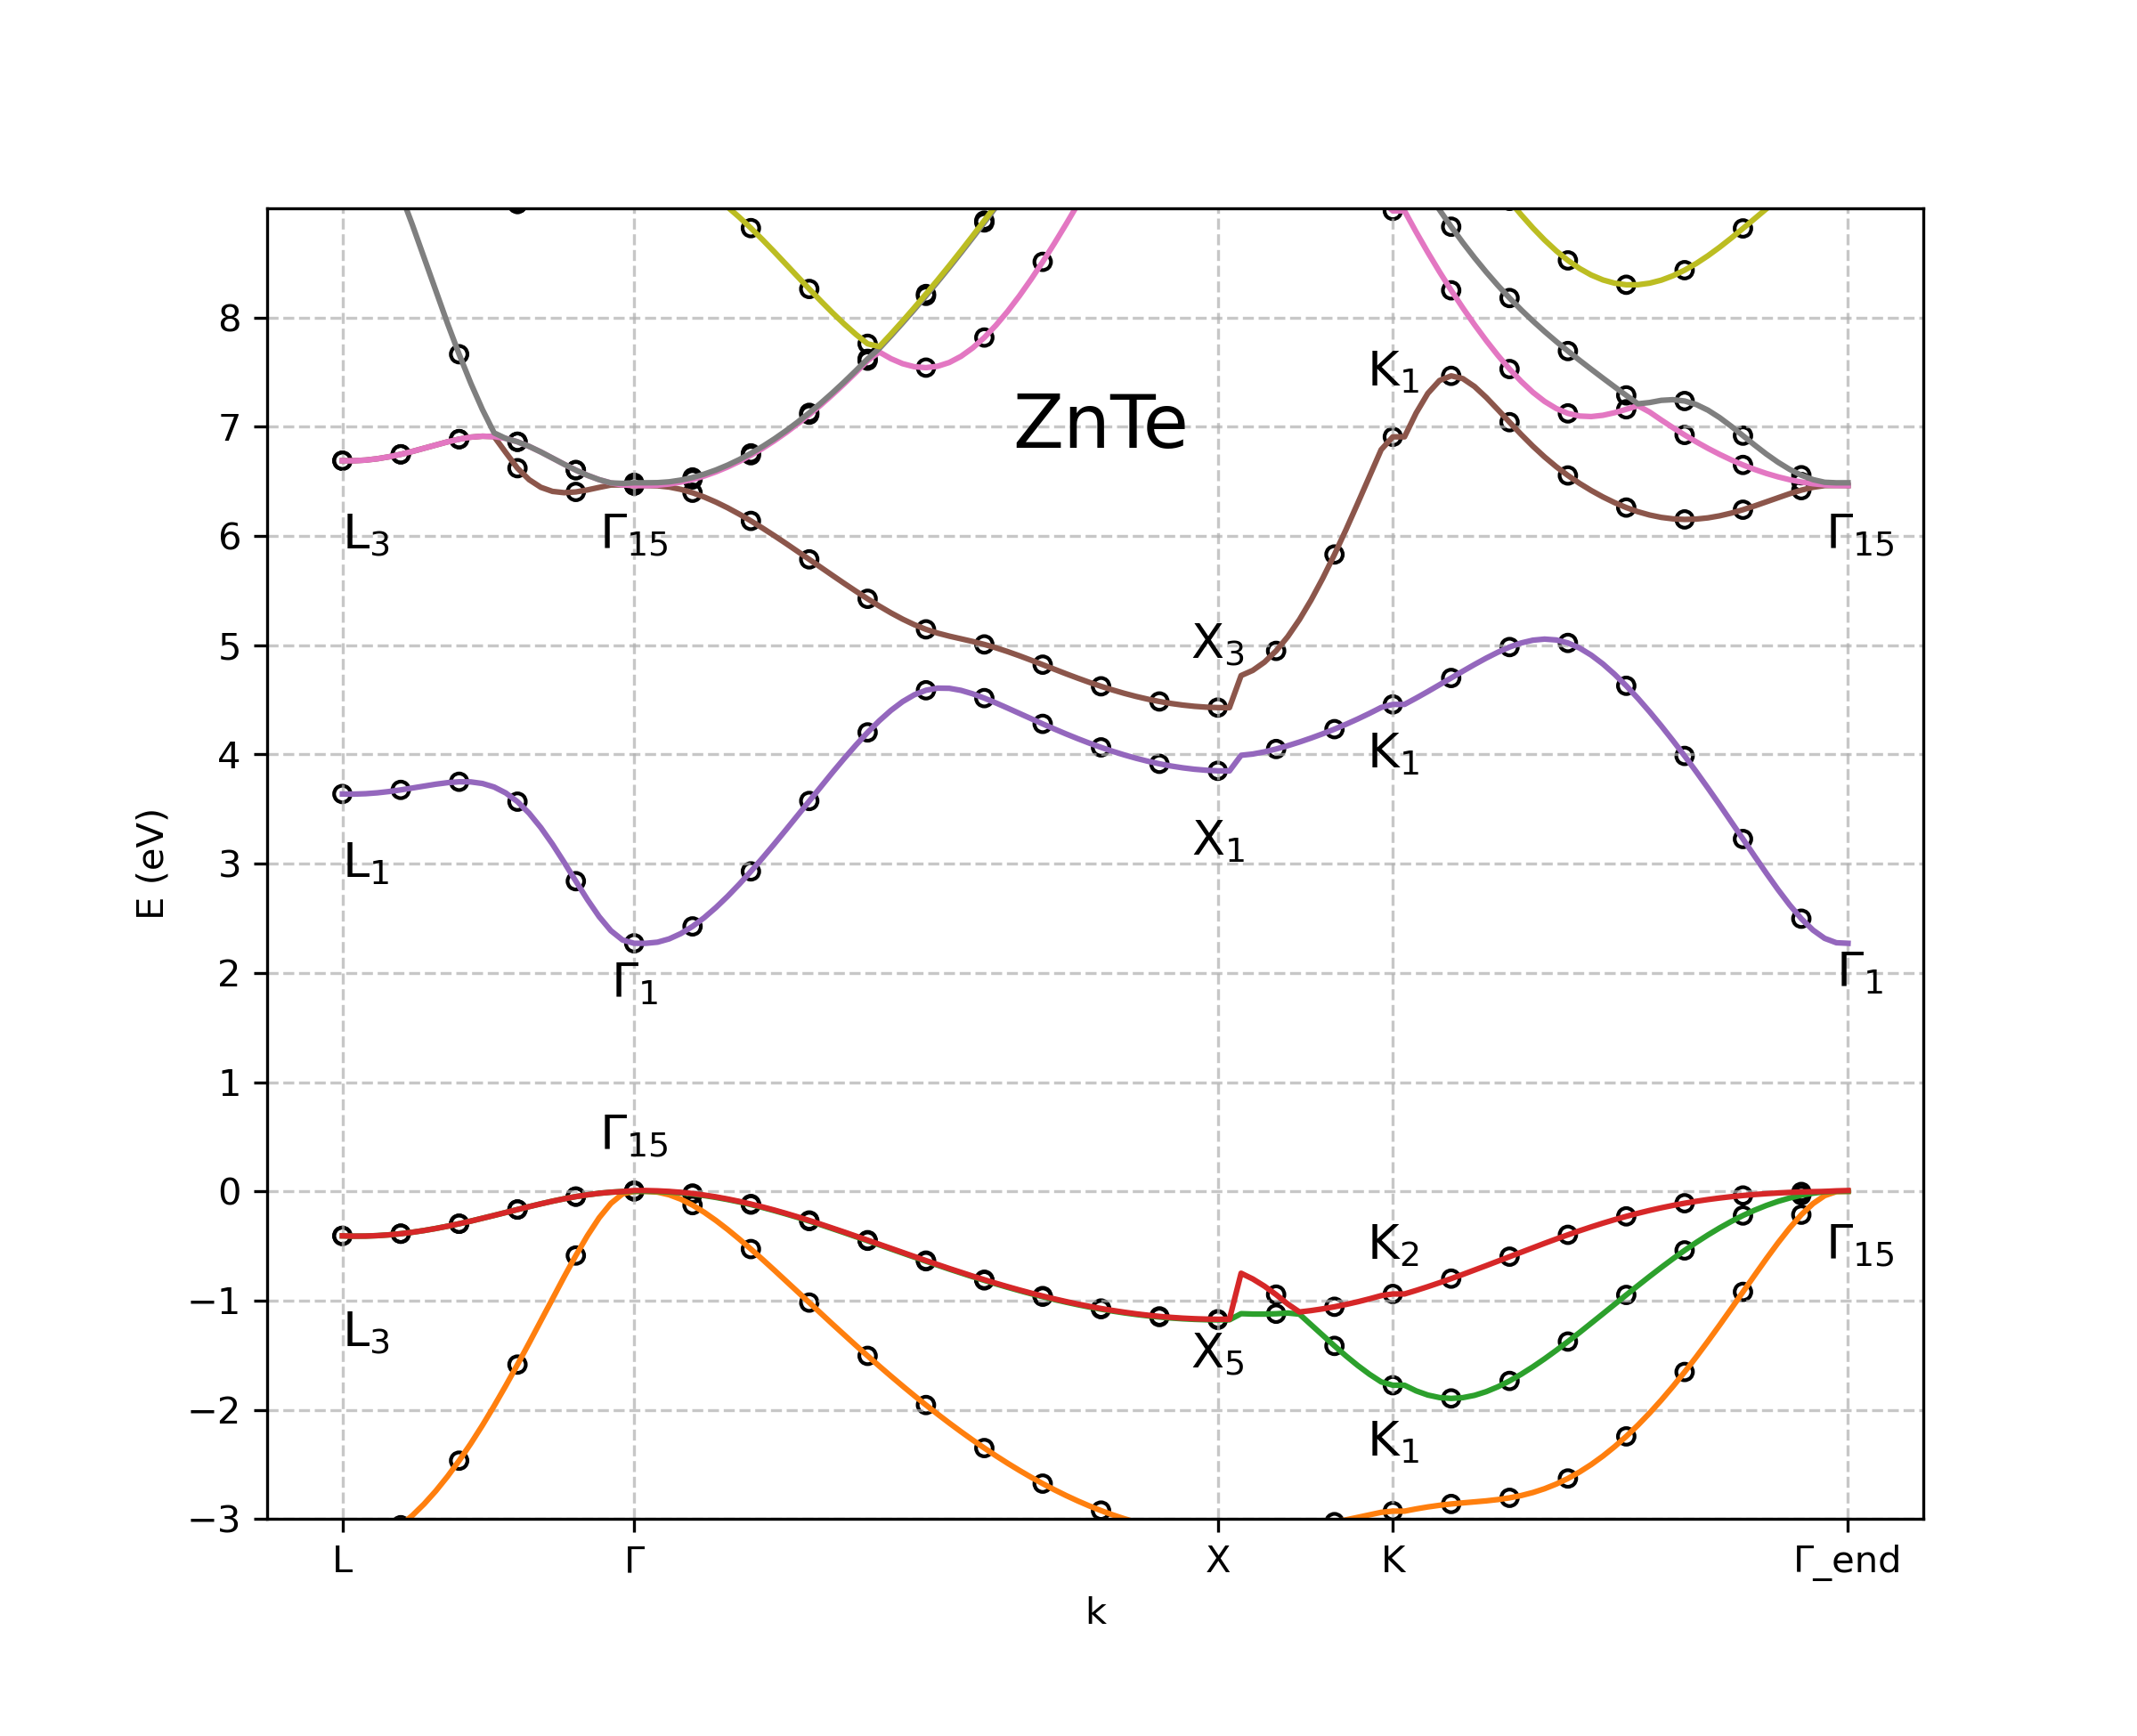
\includegraphics[width=\linewidth]{ZnTe.png}
    \vspace{-1cm}
    \caption{Band structure of ZnTe.}
    \label{fig:ZnTe}

    \centering
    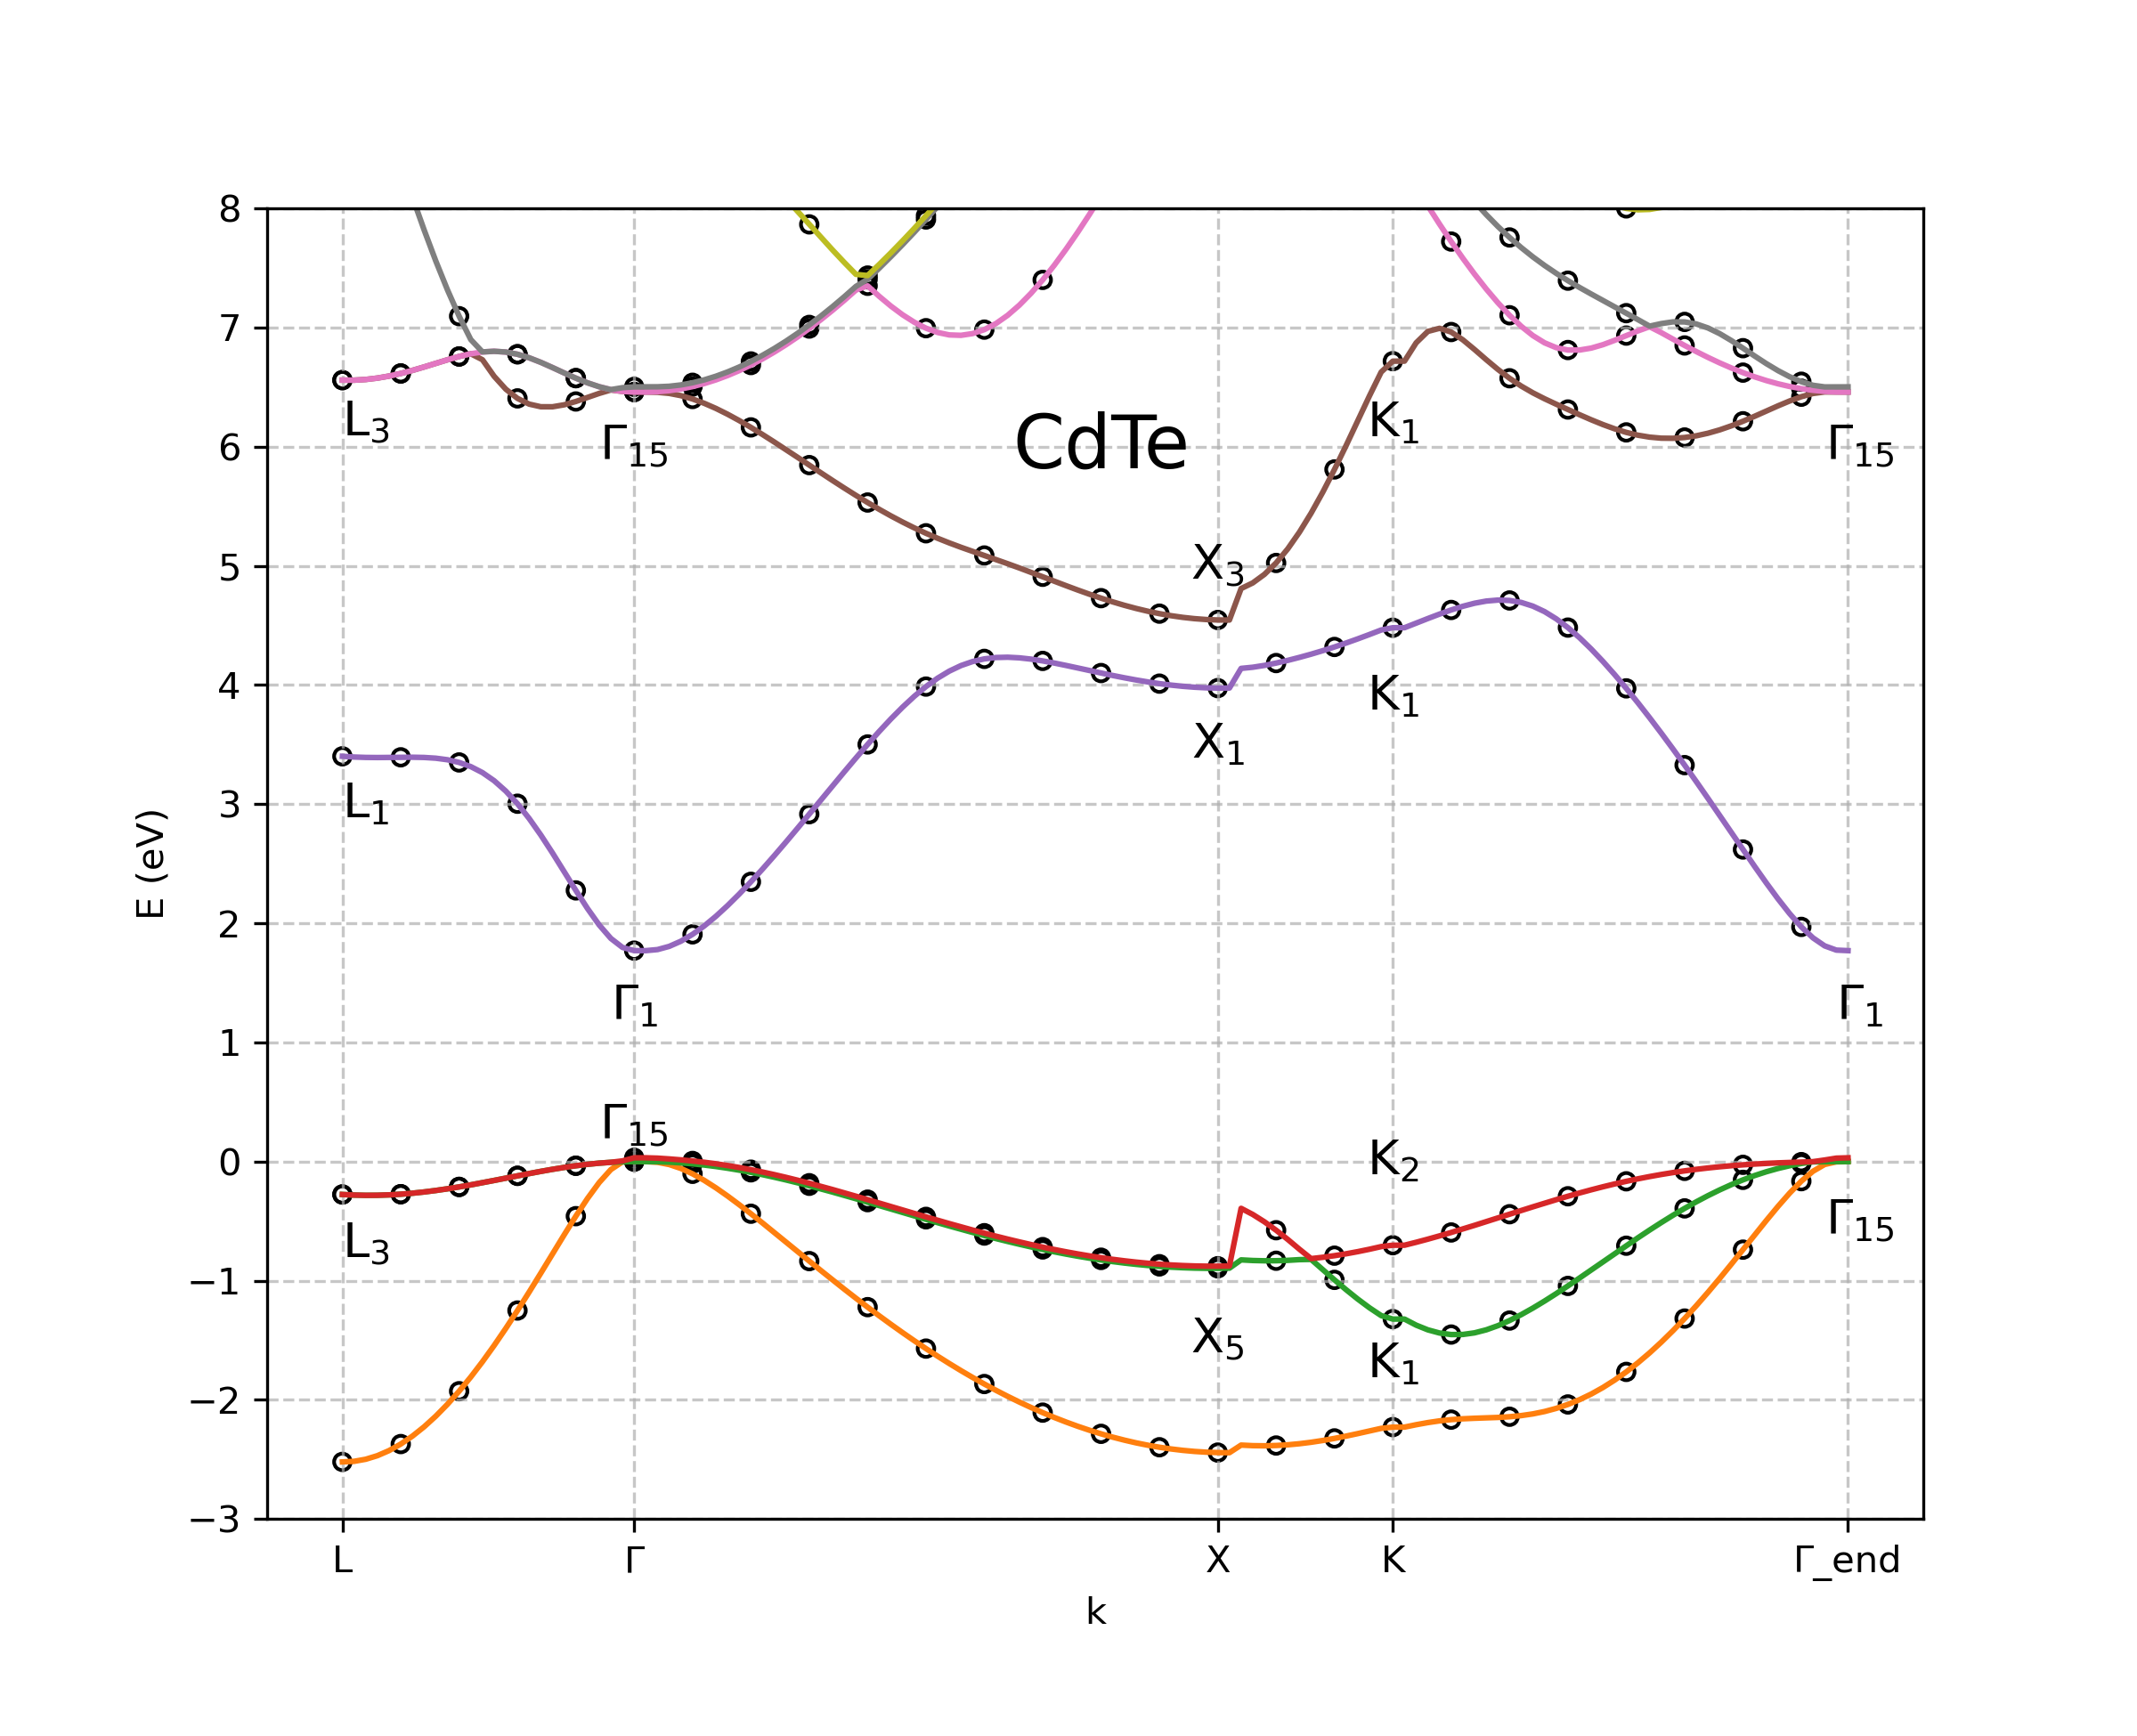
\includegraphics[width=\linewidth]{CdTe.png}
    \vspace{-1cm}
    \caption{Band structure of CdTe.}
    \label{fig:CdTe}
\end{figure}
\clearpage
\textbf{Band Structure Comparison:} The overall shapes of the band structures, including the curvature of conduction and valence bands, closely resemble those in the original study, indicating accurate representation of fundamental electronic properties. Notably, in silicon (Si), while the band gap shape mirrors that of the original work, deviations are evident at specific points, such as \( K_1 \) with an energy of 4.8 eV, compared to 5.5 eV in Cohen and Bergstresser's study.

Additionally, for Si, the second band descends and the fifth band ascends at faster rates than observed in the original research. This trend extends to other semiconductors, like InAS, InSb, and InP, suggesting variations in these specific bands compared to the original findings.

\textbf{Band Gap:} The band gaps in my plots align with those reported by Cohen and Bergstresser, albeit with minor discrepancies in several bands. Band gaps across all semiconductors demonstrate accurate energy level splitting, with differences ranging from 0.1 eV to 0.3 eV. Specifically, Sn shows a similar intersection between the third and fourth bands, and GaSb, ZnS, and ZnSe exhibit band gap structures identical to the original study. However, for CdTe, the band gap between the third band ($\Gamma_{15}$) and the fourth band ($\Gamma_1$) is 1.8 eV, slightly different from the 2 eV reported in the original study. Similarly, in Germanium (Ge), the gap between the third band ($\Gamma_{25'}$) and the fourth band ($\Gamma_{2'}$) is 1.2 eV, deviating marginally from the 1 eV in the original work.

\textbf{Feature Positioning:} The positioning of key features like peaks, valleys, and inflection points in the band structures aligns with those observed in Cohen and Bergstresser's study across the Brillouin zone. This consistency in feature positioning across all materials examined further validates the reliability of my results in comparison with the foundational research. The observed similarities in the locations of valleys, peaks, and inflection points underscore the precision of my band structure analysis.

The agreement between my results and the original plots by Cohen and Bergstresser highlights the effectiveness of the methods used in both studies. It also affirms the dependability of the electronic properties derived from these band structures, demonstrating the advancements in computational techniques for replicating key studies in solid-state physics.

\section*{4. Conclusion}

The computational analysis of 14 band structures demonstrates considerable consistency with the data from Cohen and Bergstresser. Each band's overall shape closely aligns with that of the original research, indicating reliable replication of key features. However, slight deviations in the band structures are observed, attributable to the computational advancements unavailable to Cohen and Bergstresser. These differences may also be partially due to the limitations of the original pseudoformfactor table, which contains data with only two significant digits.

Advancements in computational methods are recommended to refine the original dataset, potentially enhancing the precision of the band structure calculations for these semiconductors. 
Improved computational techniques promise more accurate representations of semiconductor band structures, thereby contributing to a deeper understanding of their electronic properties.

\section*{5. References}
[1] \textbf{Cohen, M. L., \& Bergstresser, T. K.} (1966). Band Structures and Pseudopotential Form Factors for Fourteen Semiconductors of the Diamond and Zinc-blende Structures. \emph{Phys. Rev.}, 141(2), 789--796. \url{https://link.aps.org/doi/10.1103/PhysRev.141.789}

\section*{6. Appendix}
\begin{table}[h]
    \centering
    \small
    \setlength{\tabcolsep}{4pt}
    \begin{tabular}{lrrrrrrr}
    \toprule
    Material & V0      & VS3   & VS8   & VS11  & VA3   & VA4   & VA11  \\
    \midrule
    Si       & 0.00    & -0.21 & 0.04  & 0.08  & 0.00  & 0.00  & 0.00  \\
    Ge       & -0.6951 & -0.23 & 0.01  & 0.06  & 0.00  & 0.00  & 0.00  \\
    Sn       & -0.5015 & -0.20 & 0.00  & 0.04  & 0.00  & 0.00  & 0.00  \\
    GaP      & -0.6775 & -0.22 & 0.03  & 0.07  & 0.12  & 0.07  & 0.02  \\
    GaAs     & -0.6527 & -0.23 & 0.01  & 0.06  & 0.07  & 0.05  & 0.01  \\
    AlSb     & -0.5107 & -0.21 & 0.02  & 0.06  & 0.06  & 0.04  & 0.02  \\
    InP      & -0.5627 & -0.23 & 0.01  & 0.06  & 0.07  & 0.05  & 0.01  \\
    GaSb     & -0.5112 & -0.22 & 0.00  & 0.05  & 0.06  & 0.05  & 0.01  \\
    InAs     & -0.5251 & -0.22 & 0.00  & 0.05  & 0.08  & 0.05  & 0.03  \\
    InSb     & -0.4460 & -0.20 & 0.00  & 0.04  & 0.06  & 0.05  & 0.01  \\
    ZnS      & -0.4677 & -0.22 & 0.03  & 0.07  & 0.24  & 0.14  & 0.04  \\
    ZnSe     & -0.4496 & -0.23 & 0.01  & 0.06  & 0.18  & 0.12  & 0.03  \\
    ZnTe     & -0.3925 & -0.22 & 0.00  & 0.05  & 0.13  & 0.10  & 0.01  \\
    CdTe     & -0.3117 & -0.20 & 0.00  & 0.04  & 0.15  & 0.09  & 0.04  \\
    \bottomrule
    \end{tabular}
    \caption{Form factors in Rydberg of the pseudopotentials of 14 band structures}
    \label{tab:semiconductors}
\end{table}
\end{document}
